\chapter{Numerical Techniques}\label{chap:3}
We will discuss the fundamentals of numerical methods relevant to solving the Navier-Stokes equations.
We begin the discussion of the weighted of residuals (\S \ref{sec:methodofweightedresiduals}) and the spatial discretisation using spectral/\emph{hp} element methods in one dimension (\S \ref{sec:spectralhpelementmethods}).
This is followed by techniques for solving the Navier-Stokes equations (\S \ref{sec:numeraltechniquesforNS}), introducing the velocity-correction scheme, enforcing a constant flow rate and the quasi-3D approach for semi-homogeneous domains. 
This chapter concludes with numerical techniques for the stability analysis of the Navier-Stokes equations (\S \ref{sec:stabilityanalysisofNS}), including eigenvalue computation and edge tracking.
% In this chapter, I will present the numerical methods ultilised in this thesis.
% The premise of numerical methods is to solve for the the partial differential equations, the Navier-Stokes equations.
% The incompressible Navier-Stokes equations describe the time- and spatial-varying velocity field and pressure field.
% One of the foundations of solving partial differential equations begin with the method of weighted residuals. 

%%%%%%%%%%%%%%%%%%%%%%%%%%%%%%%%%%
% 3.1 METHOD OF WEIGHTED RESIDUALS
%%%%%%%%%%%%%%%%%%%%%%%%%%%%%%%%%%

\section{Method of weighted residuals}\label{sec:methodofweightedresiduals}
Spatial discretisation errors, or residuals, arises as one seeks an approximate solution to some partial differential equation (PDE).
The method of weighted residual provides a generic mathematical framework in which constraints on the residual could be applied flexibly, defining the spatial discretisation scheme and its convergence properties.
In summary, we approximate the solution of PDE by considering a finite expansion of a suitable basis, to which its coefficients are sought after by minimising the inner product between the PDE and a test (or weight) function.
To demonstrate this, we consider a linear partial differential equation as,
\begin{equation}\label{eq:linear_operator}
    \mathbf{L}[u(x)] = 0, \quad x \in \Omega,
\end{equation}
where $\mathbf{L}$ refers to a linear spatial differential operator subjected to some boundary conditions within the domain, $\Omega$, while $u(x)$ refers to the exact solution of $\mathbf{L}$.
Examples of PDEs with linear spatial differential operators include the Laplace equation, $\nabla^2 u = 0 $, Poisson equation, $\nabla^2 u = f$, and the Helmholtz equation, $\nabla^2 u + \lambda u  = f$.
We suppose that the exact solution $u(x)$ can be approximated (discretised) by $N$ finite number of basis (or expansion) functions, $\Phi(x)$.
\begin{equation}\label{eq:approximate}
    u(x) \approx u^\delta(x) = \sum_{i=0}^{N-1} \hat{u}_i \Phi_i(x),
\end{equation}
where $u^\delta(x)$ refers to the approximate solution of $u(x)$, consisting of a linear combination of the product between the $i^{th}$ basis coefficient, $\hat{u}_i$, and the $i^{th}$ global basis expansion, $\Phi_i(x)$, defined within $\Omega$.
Since $u^\delta(x)$ is an approximate solution of equation \eqref{eq:helmholtz}, we expect a residual (or `error') between the exact solution, $u(x)$, and $u^\delta(x)$,
\begin{equation}\label{eq:residual}
    \mathbf{L}[u^\delta(x)] = R[u^\delta(x)],
\end{equation}
where $R[u^\delta(x)]$ refers to the residual which depends on the approximate solution $u^\delta(x)$ and varying within $\Omega$.
In other words, equation \eqref{eq:helmholtz} might not be satisfied everywhere in $\Omega$. 
We need to place restrictions on the residual, such that it the residual approaches zero, $R \rightarrow 0$, and the approximate solution approaches the exact solution, $u^\delta(x) \rightarrow u(x)$.
The method of residuals places a restriction on the residual by applying an inner product between the governing equation, and $N$ test (or weight) functions, $v_j(x)$, and setting it to zero,
\begin{equation}\label{eq:weightinnerresidual}
    (v_j(x), R[u^\delta(x)]) = 0, \quad j = 0, ..., N-1.
\end{equation}
\begin{definition}[Inner product]
The inner product between two functions $f(x)$ and $g(x)$ is,
\begin{equation}
       (f, g) = \int_\Omega f(x) g(x) dx \nonumber.
\end{equation}
\end{definition}
% where $(\, \cdot \, , \, \cdot \,)$ refers to an inner product, a measure of orthogonality between function $f(x)$ and $g(x)$ defined as,
% \begin{equation}\label{eq:inner-product}
%        (f, g) = \int_\Omega f(x) g(x) dx.
% \end{equation}
By setting equation \eqref{eq:weightinnerresidual} to zero, it becomes a system of $N$ ordinary differential equations, where the $N$ basis coefficients, $\hat{u}_i$.
The choice of test function defines the projection methods, and examples of projection methods are shown in table \ref{tab:weightFunction}.
We emphasise that the method of weighted residuals merely describes the projection method, but does not specify the type of basis expansions, as we will discuss later in \S \ref{sec:spectralhpelementmethods}.
The choice of projection method coupled with suitable basis expansions will have different solution convergence properties.
A particular interest is on how quickly the residual vanishes as the number of basis expansions increases.
For instance, by considering the Galerkin method coupled with Fourier expansions, one can expect exponential convergence, desirable for an efficient representation of turbulent dynamics.
% Certain mathematical properties such as spectral convergence as desired in the case of Galerkin projection using Fourier expansions, 
% The choice of \emph{trial} functions used in \emph{nektar++} will be elaborated in Section \ref{sec:modifiedBasis}.
% the method of weighted residuals is only restrictive to the weight
% Table \ref{tab:weightFunction} shows the different forms of weight functions and its corresponding numerical method.
\renewcommand{\arraystretch}{1.5} % Default value: 1
\begin{table}[h]
    \centering
        \begin{tabular}{cc}
            Weight functions & Projection method \\
            \hline
            $v_j(x) = \delta(x-x_j)$ & Collocation \\
            $v_j(x) =\left\{\begin{array}{ll}
                1 & \mbox{if } x \in \Omega_j\\
                0 & \mbox{if } x \notin \Omega_j \\
           \end{array}\right. $& Finite-Volume \\
            $v_j(x) = \phi_j$& Galerkin \\
            $v_j(x) = \frac{\partial R}{\partial \hat{u}_j}$ & Least-squares \\
            \hline
        \end{tabular}
        \caption{Examples of weight functions and projection methods}
    \label{tab:weightFunction}
\end{table}
% For instance, for $v_j = \delta(x-x_j)$, the numerical method becomes the \emph{collocation} method where the differential equation is satisfied on discrete points $x_j$.
% The type of restriction on the residual is implemented through the choice of \emph{test} function, $v_j$.
\section{Galerkin Projection}\label{sec:galerkinprojection}
The Galerkin projection remains a standard projection method in the context of the finite element method, where the test functions, $v(x)$, are chosen to be lie in the same functional space as the global basis functions, $\Phi(x)$.
To demostrate the Galerkin projection method, we consider that the differential operator earlier in equation \eqref{eq:linear_operator} as a 1D Helmholtz equation,
\begin{subequations}\label{eq:helmholtz}
    \begin{equation}
        \mathbf{L}[u(x)] \equiv \frac{\partial^2 u(x)}{\partial x^2} - \lambda u(x) - f(x) = 0, \quad x \in \Omega := [0, l]
    \end{equation}
    \begin{equation}
        u(0) = g_D, \quad \frac{\partial u}{\partial x}\Big|_{x=l} = g_{N}.
    \end{equation}
\end{subequations}
where $\lambda$ is a real positive constant, $f(x)$ is a forcing function, and $\Omega$ refers to the spatial domain bounded between $0$ and $l$. 
% $ hh u(x), \lambda, f, \Omega$ refers to the linear (spatial) differential operator, solution to the diffential equation, a real positive constant, forcing function and the spatial domain bounded between 0 and $l$, respectively.
To ensure that problem is well posed, Dirichlet and Neumann boundary conditions, $g_D$ and $g_N$, are imposed at $x = 0$ and $x = l$ respectively.
% In order for the problem to be well-posed, we impose both Dirichlet and Neumann, boundary conditions corresponding to $g_D$ and $g_N$ at $x= 0 $ and $x=l$, respectively.
Equation \ref{eq:helmholtz} is commonly referred to as the strong or classical form.

The subsequent step in Galerkin projection methods is take the inner product of the equation \eqref{eq:helmholtz} with a test function, $v(x)$, that satisfies the homogeneous Dirichlet boundary conditions by definition, i.e. $v(0) = 0$, and setting the inner product to zero,
\begin{equation}\label{eq:helmholtz_inner}
    (v(x), \, \mathbf{L}[u(x)]) = \int_0^l w\left[\frac{\partial^2 u(x)}{\partial x^2} - \lambda u(x) + f(x)\right] \mathrm{d}x =  0.
\end{equation}
This step is equivalent to applying the method of weighted residuals (\S \ref{sec:methodofweightedresiduals}), where $u(x)$ could refer to the approximate solution, $u^\delta(x)$. 
Next, we perform integration by parts,
\begin{equation}\label{eq:weak_form}
    \underbrace{\int_0^l \frac{\partial v}{\partial x}\frac{\partial u}{\partial x} \, \mathrm{d}x + \int_0^l \lambda v u \, \mathrm{d}x}_{a(v,u)}= \underbrace{\int_0^l v f \, \mathrm{d}x + \left[ v \frac{\partial u}{\partial x} \right]_0^l}_{f(v)}.
\end{equation}
This equation is typically referred to as the weak \footnote{The notions of the \emph{weak} and \emph{strong} are refers to the smoothness (regularity) required of admissible solutions. In the weak formulation, the highest derivative involved is up to first-order, so the solution space is $H^1$. This space is generally larger than that of the strong formulation, which required $u \in \mathcal{H}^2(\Omega)$. Since $H^2(\Omega) \subset H^1(\Omega)$ the weak formualation imposesd a `less stringent' constraint of the solution space of admissible functions.} form of equation \eqref{eq:helmholtz}.
In compact notation, we define the bilinear and linear forms as,
\begin{subequations}
    \begin{equation}
        a(v,u) = f(v),
    \end{equation}
\end{subequations}
where $a(v,u)$ and $f(v)$ are typically refered to as the strain energy and forcing function in structural mechanics, required to remain finite.
To ensure this, we restrict the choice of solutions $u(x)$ to lie in the solution space, $\mathcal{U}$, defined as
\begin{equation}\label{eq:solution_space}
    \mathcal{U} := \{ u \, | \, u \in H^1(\Omega), u(0) = g_D \},
\end{equation}
% where $u \in H^1$ contains functions of $u$ in the Sobolev space such that the Dirichlet condition $u(0) = g_D$ is statisfied and the sum of square integral of $u$ and its first derivatives, $\frac{\partial u}{\partial x}$ remains bounded,
where $u \in H^1$ refers to functions of $u$ belonging to Sobolev space of order 1, and satistfying the Dirichlet condition, $u(0) = g_D$,  at $x = 0$.
\begin{definition}[Sobolev space]
    We define Sobolev space of order $n \geq 1$ on $\Omega$,
    \begin{equation}
        H^n(\Omega) = \{u \, | \, u \in L_2(\Omega), D^\alpha u \in L_2(\Omega), \forall \alpha : \alpha \leq n\}, \nonumber
    \end{equation}
    where $D^\alpha u$ refers to derivatives up to order $\alpha$ and $L_2(\Omega)$ refers to functions that are square integrable.
\end{definition}
\begin{definition}[$L_2$ space]
    The space $L_2(\Omega)$ refers to functions that are square integrable,
    \begin{equation}
        (u, u)_{L_2} = \int_\Omega |u(x)|^2 \, \mathrm{d}\Omega < \infty. 
    \end{equation}
\end{definition}
We consider admissible functions up to the first derivatives, the highest order derivative in the weak formulation of equation \eqref{eq:helmholtz_inner}.
Similarly, the space of test functions, $\mathcal{V}$, is defined as,
\begin{equation}\label{eq:test_space}
    \mathcal{V} := \{ v \, | \, v \in H^1, v(0) = 0 \},
\end{equation}
where $v \in H^1$ are refer to test functions belonging to the Sobolev the space of order 1, and is defined to be zero, $v(0) = 0$ on Dirichlet boundary condition, $x = 0$.
The generalised weak form is therefore finding $u(x) \in \mathcal{U}$, such that
\begin{equation}\label{eq:bilinear_infinite}
    a(v,u) = f(v), \quad \forall v \in \mathcal{V}.
\end{equation}
At this point, equation \eqref{eq:bilinear_infinite} is infinite dimension as the function spaces, $\mathcal{U}$ and $\mathcal{V}$, contain infinitely many functions.
% This formulation is infinite dimensional, as the function space $\mathcal{U}, \mathcal{W}$ contain infinitely many functions.
To obtain an approximate solution, $u^\delta(x)$, we restrict ourselves to finite dimensional subspaces, $\mathcal{U}^\delta \subset \mathcal{U}$, and $\mathcal{V}^\delta \subset \mathcal{V}$.
The problem is then to find $u^\delta \in \mathcal{U}^\delta$, such that
\begin{equation}
    a(v^\delta, u^\delta) = f(v^\delta), \quad v^\delta \in \mathcal{V}^\delta.
\end{equation}
Here, the subspaces $u^\delta \in \mathcal{U}^\delta$ and $v^\delta \in \mathcal{V}^\delta$ are not the same, compare equations \eqref{eq:solution_space} and \eqref{eq:test_space}, necessary for the standard Galerkin projection procedure where they should lie in the same subspace.
To ensure that they belong to the same space, we lift the solution $u^\delta$ into two parts,
\begin{equation}
    u^\delta = u^\mathcal{H} + u^\mathcal{D}.
\end{equation}
where $u^\mathcal{H} \in \mathcal{V}^\delta$ satisfies the homogeneous Dirichlet condition (e.g. is zero on Dirichlet boundaries), belonging to the same subsapce as $v^\delta \in \mathcal{V}^\delta$, while $u^\mathcal{D} \in \mathcal{U}^\delta$ satisfies the Dirichlet boundary conditions $u^\mathcal{D}(0) = g_D$.
Hence, the standard Galerkin projection method is to search for the homogeneous solution, $u^\mathcal{H} \in \mathcal{V}^\delta$, such that,
\begin{equation}\label{eq:standard_galerkin}
    a(v^\delta, u^\mathcal{H}) = f(v^\delta) - a(v^\delta, u^\mathcal{D}).
\end{equation}
This concludes the classical Galerkin formulation. 
Under certain assumptions of $a$, a solution is guaranteed under the Lax-Milgram theorem \citep{bers_ix_1955}.
%%%%%%%%%%%%%%%%%%%%%%
% SPECTRAL/HP ELEMENTS
%%%%%%%%%%%%%%%%%%%%%%

\section{Spectral/\emph{hp} element method}\label{sec:spectralhpelementmethods}
We have described the procedure for approximating a solution of a PDE using the classical Galerkin projection technique.
However, the spatial discretisation scheme, related to the choice of basis (and test) functions, remains undiscussed.
% and describe the essential numerical differential and integral techniques.
% , equation \eqref{eq:standard_galerkin} reduces to a system of linear equations.
% To represent the spatially-dependent velocity and pressure fields, spatial discretisation is performed using the spectral/\emph{hp} element method.
% Other popular methods of spatial discretisation found in literature are the finite-difference methods, and finite-volume methods.
% The spectral/{hp} element method (SEM) is related to the Galerkin method in which the type of \emph{trial} function used. The spectral/\emph{hp} element method combines 2 traditional numerical methods, namely, 
In this section, we discuss the spectral/\emph{hp} element method \citep{patera_spectral_1984},
where the solution is partitioned into a set of non-overlapping finite elements of size $h$, consisting of a linear combinbation of continuous orthogonal polynomial functions up to order $P$.
% The spectral/\emph{hp} element method pioneered by \citep{patera_spectral_1984} is a spatial discretisation technique in which the solution domain is partitioned into a set of non-overlapping (finite) elements with size $h$, each consisting of a linear combination of continuous polynomial functions of up to order $P$. 
% represented by a polynomial of up to order $p$.
% which leverages the advantages of offering geometric flexibility by decomposing the global domain into a set of non-overlapping (finite) elements of size $h$, each consisting of a linear combination of continuous polynomial functions of up to order $p$.
It leverages the geometric flexibility of classical finite-element methods, allowing for the representation of complex engineering geometries, and the exponential (spectral) convergence properties of classical spectral methods, where the solution error decreases exponentially.
% The Spectral/\emph{hp} element method leverages the advantages of both methods - geometric flexibility and spectral covergence.
% The spectral/\emph{hp} method uses a series of high-order polynomials (Lagrange/Legendre) within each element.
Suppose we consider $P+1$ linearly independent polynomials spanning the polynomial space of $\mathcal{P}_P$, the error of a smooth solution with element size of $h$ and polynomial order $P$ has the property of \citep{karniadakis_spectralhp_2005}, 
\begin{equation}\label{eq:error_convergence}
    ||u(x) - u^{\delta}(x)|| \leq Ch^P||u(x)|| \approx O(h^P).
\end{equation}
where $C$ is some constant.
Equation \ref{eq:error_convergence} implies that the error decreases linearly with $h$, and exponentially with $P$.
This section is organised into domain partition, standard elements, assembly process, modal and nodal expansion functions, numerical integration and differentiation, concluding with an example in 1D.
% % It offers the flexibility of offering refinements in either $h$ or $p$, or both.
% \begin{enumerate}
%     \item Finite elements:
%         \subitem The finite element method decomposes the global domain into a set of non-overlapping subdomains (finite elements), represented by linear shape functions. In a 1D domain, the size of each element is given by $h$ and the approximate solution should covergence as $h$ is decreased - also known as \emph{h}-refinement. The flexibility of domain decomposition allows for complex engineering geometries to be represented. 
%     \item Spectral method:
%         \subitem The spectral method performs a global discretisation of the domain. The domain is represented by a linear combination of global continuous functions, such as the Fourier series. Spectral methods benefit from the property of \emph{spectral convergence}, where the solution error decreases by $\mathcal{O}(c^{-N})$, where $c$ is some constant $0 \leq c \leq 1$ and $N$ is the number of polynomials (\cite{trefethen_2000}). In other words, as the number of functions is increased, the error decreases exponentially.
% \end{enumerate}

%%%%%%%%%%%%%%%%%%
% DOMAIN PARTITION
%%%%%%%%%%%%%%%%%%
\subsection{Domain partition}
The first step concerns the partitioning the domain into a set of (finite) elemental regions.
We consider an example in one dimension within $\Omega$, and partition it into a set of $N_{el}$ elements, where $\Omega^e$, refers to the elemental partitions with $1 \geq e \geq N_{el}$, such that they meet at their boundaries and do not overlap,
\begin{equation}
    \Omega = \bigcup_{e = 1}^{N_{el}} \Omega^e, \quad \text{where} \; \bigcap_{e=1}^{N_{el}} \Omega^e = \emptyset
\end{equation}
where the $e^{th}$ element is defined as,
\begin{equation}
    \Omega^e = \{x \, | \, x_{e-1} \geq x \geq x_e \}.
\end{equation}
Each element can be represented by a linear combination of orthogonal basis expansions.
The basis expansions can be either modal or nodal expansions, as we shall see later.
% Each element it then represented by a linear combination, $\phi(x)$, where $x$ is referred to the \emph{global} domain.

%%%%%%%%%%%%%%%%%%%
% STANDARD ELEMENTS
%%%%%%%%%%%%%%%%%%%
\subsection{Standard Elements}
\begin{figure}[h]
    \centering
    \includegraphics[width=\textwidth]{NumericalMethods/Figures/standard_element_3elements.pdf}
    \caption{A spectral/\emph{hp} element representation of $u(x)$, consisting of three non-overlapping finite elements, each containing a linear combination of local expansion bases of up to $P=2$.}
    \label{fig:standard_element}
\end{figure}
In general, we expect to work with non-uniform elements that may have arbitrarily shapes, making the definition of basis expansions potentially unwieldy.
To simplify the formulation, it is convenient to define a \textit{standard} element,
\begin{equation}
    \Omega_{st} = \{ \xi \, | \, -1 \geq \xi \geq 1 \},
\end{equation}
where $\Omega_{st}$ refers to the standard element defined in local coordinates, $\xi \in [-1, 1]$.
Within this standard element, the formulation of basis expansions, as well as differential and integration operations, can be carried out in the local coordinate system $\xi$, before mapping the solution back to the global domain, $x$.
We can map the standard element into any arbitrary global coordinates based on a linear mapping $\chi^e:\Omega_{st} \rightarrow \Omega$,
\begin{equation}
    x = \chi^e(\xi) = \frac{1-\xi}{2} x_e + \frac{1 + \xi}{2}x_{e+1}, \quad \xi \in \Omega_{st}
\end{equation}
which has an analytical inverse, $(\chi^e)^{-1}(x)$,
\begin{equation}
    \xi = (\chi^e)^{-1}(x) = 2 \frac{x - x_{e-1}}{x_e - x_{e-1}} - 1, \quad x \in \Omega^{e}.
\end{equation}
For illustration purposes, we consider that the standard element can be represented by three local basis expansions of polynomial order of up to $P = 2$,
\begin{equation}\label{eq:def_local_expansions}
    \phi_0^e(\xi) = \frac{1 - \xi}{2}, \quad \phi_1^e(\xi) = (1 + \xi)(1 - \xi), \quad \phi_2^e(\xi) =  \frac{1 + \xi}{2},
\end{equation}
where $\phi_0^e, \phi_2^e$ and $\phi_1^e$ refers to the linear and quadratic local basis expansions of the $e^{th}$ element.
These local basis expansions is illustrated in figure \ref{fig:standard_element}.
We note that the formulations of local basis expansion here is merely an example.
In practice, the local basis expansions are usually chosen to have orthogonality properties under a certain inner product.
The approximate solution is now represented as,
\begin{equation}\label{eq:local_expansions}
    u^\delta(x) = \sum_{e=0}^{N_{el}-1}\sum_{i=0}^P \hat{u}_i^{e}\phi^e_i(\chi^e(\xi)).
\end{equation}
where $\hat{u}_i^e$ refers to the local expansion basis coefficients.
The approximate solution, $u^\delta(x)$, now lie within the solution space $\mathcal{U}^\delta$ defined as,
\begin{equation}
    \mathcal{U}^\delta := \left\{ u^\delta \,\middle|\, u^\delta \in H^1,\ u^\delta(\chi^e(\xi)) \in \phi_i^e(\xi), \forall i : 0 \leq i \leq P, \forall e : 0 \leq e \leq N_{el} \right\}
\end{equation}
% Figure \ref{fig:standard_element} presents the sketch of representing a continous function using spectral/\textit{hp} element methods for $P = 2$ and $N_{el} = 3$.

%%%%%%%%%%%%%%%%%%%%
% ASSEMBLY FUNCTIONS
%%%%%%%%%%%%%%%%%%%%

\subsection{Global assembly}
In this section, we introduce the concept of global assembly (or direct stiffness summation) which relates the global basis expansions (equation \eqref{eq:approximate}), $\Phi_i(x)$, to the local basis expansions (equation \eqref{eq:local_expansions}), $\phi_i^e(x)$, where the solution can be approximated using either formulation,
\begin{equation}
    u^\delta(x) = \sum_{i=0}^{N-1}\hat{u}_i\Phi_i(x) = \sum_{e=0}^{N_{el}-1}\sum_{i=0}^P \hat{u}_i^{e}\phi^e_i(\chi^e(\xi)).
\end{equation}
In general, we can represent the global and local basis coefficients each as a column vector,
\begin{equation}
    \mathbf{\hat{u}}_g = 
\begin{pmatrix}
    \hat{u}_0 \\
    \vdots \\ 
    \hat{u}_N
\end{pmatrix},
\quad 
\mathbf{\hat{u}}_l = 
 \begin{pmatrix}
     \mathbf{\hat{u}}^0 \\ 
     \vdots \\
     \mathbf{\hat{u}}^{N_{el}-1}
 \end{pmatrix},
\end{equation}
where $\mathbf{\hat{u}}^{e} = (\hat{u}_0^e, ..., \hat{u}_P^e)^T$, $\mathbf{\hat{u}}_g \in \mathbb{R}^N$, $\mathbf{\hat{u}}_l \in \mathbb{R}^{N_{loc}}$ and $N_{loc} = N_{el}(P+1)$.
As there can be more global degrees of freedom than local degrees of freedom, $N > N_{loc}$, we need to impose some conditions on the local expansion coefficients.
One of the common approach is to enforce $C^0$ continuity across elemental boundaries, referred to as the continous Galerkin projection.
Following the definition of local basis expansions in equation \eqref{eq:def_local_expansions}, this condition can be supplemented using,
\begin{equation}
    \hat{u}^{e-1}_P = \hat{u}^e_0.
\end{equation}
\begin{figure}[h]
\centering
\includegraphics[width=\textwidth]{NumericalMethods/Figures/standard_element_3elements_C0.pdf}
\caption{A graphical representation of $C^0$ across elemental boundaries and the relationship between local basis coefficients, $u_0^e, u_P^e$, and global basis expansions, $u_i$.}
\label{fig:local_to_global}
\end{figure}
The graphical representation of this condition enforcing $C^0$ continuity between the element boundaries for three finite elements with $P=2$ local basis expansions, and the relationship between global and local basis coefficients are shown in figure \ref{fig:local_to_global}.
% In the approach of continuous Galerkin projection methods, we enforce our solution to be $C^0$ continuous across the elemental boundaries.
% In other words, the neighbouring linear interior elements must meet at the boundaries, such that the local expansion coefficients are constrained by,
% We can ultilise a mapping b
We can relate the global and local basis coefficients with an assembly matrix, $\mathbf{A} \in \mathbb{R}^{N_{loc} \times N}$,
% This constraint by consider a mapping between the (global) expansion coefficients, and local expansion coefficients, 
% Due to the constraint described above, we need a mathematical process which maps the local coefficients to the global coefficients.
% To fulfil this description, we introduce a vector of global coefficients, $\mathbf{\hat{u}}_g$, and local coefficients $\mathbf{\hat{u}}_l$, and a linear map $\mathbf{A}$, given as,
% In this case, we introduce the definition of global modes given as,
% \begin{equation}
%     u^\delta(x) = \sum_{i=0}^{N_{dof}-1} \hat{u}_i \Phi_i(x) = \sum_{e=1}^{N_{el}}\sum_{i=0}^P \hat{u}_i^{e}\phi^e_i(\chi^e(\xi)).
% \end{equation}
% where $\Phi_i(x)$ refers to global modes, that is defined in the entire domain.
\begin{equation}
    \mathbf{\hat{u}}_l = \mathbf{A} \mathbf{\hat{u}}_g.
\end{equation}
In the case for $P=2$ and three finite elements as in the case of figures \ref{fig:standard_element}and \ref{fig:local_to_global}, the assembly matrix and the vectors of global and local basis coefficients are given as,
\begin{equation}
    \begingroup
    \setlength\arraycolsep{2pt}
    \renewcommand{\arraystretch}{1} % Smaller line spacing
        \mathbf{\hat{u}}_l = 
        \begin{pmatrix}
            \hat{u}_0^0  \\
            \hat{u}_1^0  \\
            \hat{u}_2^0  \\
            \hat{u}_0^1  \\
            \hat{u}_1^1  \\
            \hat{u}_2^1  \\
            \hat{u}_0^2  \\
            \hat{u}_1^2  \\
            \hat{u}_2^2  \\
        \end{pmatrix},
        \quad
        \mathbf{A} = 
        \begin{pmatrix}
            1 & 0 & 0 & 0 & 0 & 0 & 0\\
            0 & 1 & 0 & 0 & 0 & 0 & 0\\
            0 & 0 & 1 & 0 & 0 & 0 & 0\\
            0 & 0 & 1 & 0 & 0 & 0 & 0\\
            0 & 0 & 0 & 1 & 0 & 0 & 0\\
            0 & 0 & 0 & 0 & 1 & 0 & 0\\
            0 & 0 & 0 & 0 & 1 & 0 & 0\\
            0 & 0 & 0 & 0 & 0 & 1 & 0\\
            0 & 0 & 0 & 0 & 0 & 0 & 1\\
        \end{pmatrix}
        ,
        \quad 
        \mathbf{\hat{u}}_g
        \begin{pmatrix}
            \hat{u}_0  \\
            \hat{u}_1  \\
            \hat{u}_3  \\
            \hat{u}_4  \\
            \hat{u}_5  \\
            \hat{u}_6  \\
        \end{pmatrix},
    \endgroup
\end{equation}
% where $\mathbf{\hat{u}}_l, \mathbf{\hat{u}}_g, \mathbf{A} \in \mathbb{R}^{N_l, N_g}$ refers to the vector of local, global expansion and scatter matrix, and $N_l = N_{el} \times (P + 1)$ refers to the total local degrees of freedom while $N_g = N_l - (N_{el} - 1)$, the global degrees of freedom.
The assembly matrix $\mathbf{A}$ `scatters' the global degrees of freedom to local degrees of freedom, while the transpose of it, $\mathbf{A}^T$, performs the reverse, referred to as global assembly.
% , is known as an assembly operation, assembling local degrees of freedom to global degrees of freedom.
For example, we wish to perform integration in the domain $\Omega$, 
\begin{equation}
    \mathbf{I}_g[j] = (\Phi_j(x), u^\delta(x)),
\end{equation}
where $\mathbf{I}_g \in \mathbb{R}^{N}$ refers to a vector containing the integral between $\Phi_i(x)$ and $u^\delta(x)$.
This is related to first performing integration using local expansion basis within standard elements, and then assembling using $\mathbf{A}^T$,
\begin{subequations}
    \begin{equation}
        \mathbf{I}_g = \mathbf{A}^T \mathbf{I}_l,
    \end{equation}
    \text{where,}
    \begin{equation}
    \mathbf{I}_g =  
    \begin{bmatrix}
        \mathbf{I}_0 \\
        \vdots \\
        \mathbf{I}_{N_g-1}
    \end{bmatrix}
    ,
    \quad 
    \mathbf{I}_l =  
    \begin{bmatrix}
        \mathbf{I}^0 \\
        \vdots \\
        \mathbf{I}^{N_{el}-1}
    \end{bmatrix}
    ,\quad \text{with} \quad
    \mathbf{I}^e =  
    \begin{bmatrix}
        \int_{-1}^1 \phi_0^e(\xi) u(\chi^e)\frac{\mathrm{d} \chi^e}{\mathrm{d} \xi}\, \mathrm{d}\xi \\
        \vdots \\
        \int_{-1}^1 \phi_{P-1}^e(\xi) u(\chi^e)\frac{\mathrm{d} \chi^e}{\mathrm{d} \xi}\, \mathrm{d}\xi
    \end{bmatrix},
    \end{equation}
\end{subequations}
and $\mathbf{I}_l \in \mathbb{R}^{N_{loc}}$ refer to the vector of integration operations performed within a standard element.
In the spectral/\textit{hp} element approach, we perform integration and differentiation using local basis expansions within a standard element.
After doing so, we assemble the local operations from the standard element to the global domain by using $\mathbf{A}^T$, as we shall show later using a 1D example.
We note that the structure of assembly matrix is generally sparse, where the entries either contain 0, 1 or -1 in multidimensional formulation.
Therefore, the assembly matrix is not constructed in practice, and a mapping array is used instead.

% \begin{equation}
%     \mathbf{I}_g[j] = (\Phi_j(x), u^\delta(x)) = \int_\Omega \Phi_j(x) \, \sum_{i=0}^P\sum_{e=0}^{N_{el} -1} \hat{u}_i^e\phi_i^e(\chi^e(\xi)) \, \mathrm{d} x
% \end{equation}



%%%%%%%%%%%%%%%%%
% BASIS FUNCTIONS
%%%%%%%%%%%%%%%%%

\subsection{Local basis expansions}
The choice of local basis expansions, $\phi_i^e(\xi)$, concerns the representation of the solution, and the convergence properties of the numerical solver, in particular, the condition number of the mass and laplacian matrices.
In general, the the local basis expansions can be classified into two groups, either \textit{modal} or \textit{nodal} expansions.
% Here, we discuss the expansion functions of $\phi(\xi)$, where in general could be categorised into \emph{modal} (hierarchical) expansions or \emph{nodal} expansions.

% Modal expansions
\subsubsection{Modal expansions}
Modal expansions, or hierarchical expansions, describes a set of expansion basis where an expansion set ($\mathcal{X}_{P-1}^\delta$) of order $P-1$, is contained within a set ($\mathcal{X}_P^\delta$) of order $P$, e.g. $\mathcal{X}_{P-1}^\delta \subset \mathcal{X}_P^\delta$.
An example of modal expansions are the Jacobi polynomials, $P_p^{\alpha,\beta}(x)$, representing a family of solutions to the Sturm-Liouville problem within, $x \in [-1, 1]$.
The Jacobi polynomials become symmetric for $\alpha = \beta$, referred to ultraspheric polynomials. 
Special cases of ultraspheric polynomials are the Legendre polynomials, $\alpha = \beta = 1$, and the Chebyshev polynomials, $\alpha = \beta = 1/2$.
% Notably, the Legendre polynomials are a special case of Jacobi polynomials, $L_n(\xi) = P_n^{0,0}(\xi)$ with $\alpha = \beta = 0$.
% The \emph{trial} functions $\phi_p$ (or basis expansions) used in spectral/\emph{hp} method consist of \emph{boundary} and \emph{interior} modes.
% \emph{Interior} modes are defined to be zero on all boundaries, and non-zero within the boundary, satisfying homogeneous boundary conditions.
% \emph{Boundary} modes take on non-zero values on the boundary, satisfying non-homogeneous boundary conditions and providing $C^0$ continuity between elements (\cite{karniadakis_2005spectral}).
Within the Nektar++ framework, we utilise the \emph{modified} basis, constructed using on the Jacobi polynomials and modified (hence its name) by linear expansions given as,
% are used as the \emph{trial} functions. Using $\alpha=1$, $\beta=1$, and linear basis functions as \emph{boundary} modes, the modified Jacobi polynomials are,
\renewcommand{\arraystretch}{1.5} % Default value: 1
\begin{equation}\label{eq:modifiedJacobi}
    \phi_p(\xi) \rightarrow \psi_p(\xi) = \left\{
            \begin{array}{ll}
                \frac{1-\xi}{2} & \mbox{for } p=0\\
                \left(\frac{1-\xi}{2}\right)\left(\frac{1+\xi}{2}\right){P}_{p-1}^{1,1}(\xi)\righ & \mbox{for }  0 < p < P \\
                \frac{1+\xi}{2} & \mbox{for } p=P,
           \end{array}\right.
\end{equation}
We note that $\phi_p(\xi)$ refers to a general local expansion basis while $\psi_p(\xi)$ to definition of the modified basis.
\begin{figure}
    \centering
    \includegraphics[width=\textwidth]{NumericalMethods/Figures/modifiedBasis_1D.pdf}
    \caption{The modified basis for up to $P=5$ normalised to $-1 \leq \psi_p \leq 1$.}
    \label{fig:modified_basis}
\end{figure}
The one-dimensional expansion modes of the modified basis of up to $P=5$ is shown in figure \ref{fig:modified_basis}.
The linear modes, corresponding to $p = 0$ and $p = P$, are the only expansions which has a magnitude of at the boundaries, referred to as boundary modes.
The modified basis for $0 < p < P$, are clearly hierarchical, and have non-zero values except at the boundaries, referred to as interior/bubble modes.

% Nodal expansions
\subsubsection{Nodal expansions}
Nodal expansions are basis expansions that are non-hierchical, $\mathcal{X}_{P-1}^\delta \not\subset \mathcal{X}_P^\delta$.
An example of nodal expansions are the Lagrange polynomials,
\begin{equation}
    \phi_p(\xi) \rightarrow h_p(\xi) = \frac{\prod_{q = 0, q \neq p}^P (\xi - \xi_q)}{\prod_{q = 0, q \neq p}^P (\xi_p - \xi_q)}
\end{equation}
The Lagrange polynomials, $h_p(\xi)$, are particular attractive as it has a unit value at discrete nodal values, $\xi_q$, and zero everywhere else, $h_p(\xi_q) = \delta_{pq}$, which implies that
\begin{equation}
    u^\delta(\xi_q) = \sum_{p=0}^{P} \hat{u}_ph_p(\xi_q) = \sum_{p=0}^{P} \hat{u}_p\delta_{pq} = \hat{u}_q,
\end{equation}
where the Lagrange coefficient $\hat{u}_q$ is the same as the value evaluated at the node $\xi_q$.
The nodal values, $\xi_q$, are based on the Gauss-Lobatto-Legendre (GLL) points which will be defined later in \S \ref{sec:Gaussian_quadrature}.
Figure \ref{fig:Lagrange_basis} presents Lagrange expansions evaluated along the GLL points.
\begin{figure}[h]
    \centering
    \includegraphics[width=\textwidth]{NumericalMethods/Figures/Lagrange_1D.pdf}
    \caption{Lagrange polynomials for $P = 5$ with nodal values along GLL points.}
    \label{fig:Lagrange_basis}
\end{figure}
\subsubsection{Multi-dimensional expansions}
We have introduced modal and nodal expansions in one dimension, and its extension to multi-dimensions bases can be generalised using a tensorial expansion of the local expansion bases. 
The standard element in a quadrilateral, $\mathcal{Q}^2$, and a hexahedral $\mathcal{H}^3$,
\begin{equation}
    \mathcal{Q}^2 = \{-1 \leq \xi_1, \xi_2 \leq 1 \}, \quad \mathcal{H}^2 = \{-1 \leq \xi_1, \xi_2, \xi_3 \leq 1 \}
\end{equation}
where $\xi_1, \xi_2, \xi_3$ refers to the local coordinates in multi-dimensions.
The tensorial bases for quadrilaterals and hexadrals using modified bases are
\begin{equation}
    \phi_{pq}(\xi_1, \xi_2) =\psi_q(\xi_1)\psi_q(\xi_2), \quad \text{and} \quad
    \phi_{pqr}(\xi_1, \xi_2, \xi_3) =\psi_q(\xi_1)\psi_q(\xi_2)\psi_r(\xi_3).
\end{equation}
\begin{figure}[h]
    \centering
        \includegraphics[width=\textwidth]{NumericalMethods/Figures/modifiedBasis.pdf}
        \caption{Two dimensional modified basis with $p = q = 4$ in a standard quadrilateral, $-1 \leq \xi_1,\xi_2 \leq 1$. The modified bases are normalised to $-1 \leq \phi_{pq} \leq 1$.}
        \label{fig:TensorialModifiedbasis}
\end{figure}
An example of the modal tensorial bases, for $p = q = 4$ in a standard quadrilateral element in shown in figure \ref{fig:TensorialModifiedbasis}.
While we have discussed the tensorial the expansions for regular domains such as the standard quadrilateral and hexahedral elements, the extensions for simplex domains such as triangles, tehtrahedrals, prisms and pyramids commonly used to represent complex geometries, are less straightforward.
The challenge for simplexes is that the local coordinates, $\xi_1,\xi_2,\xi_3$, become dependent where a direct tensorial expansion becomes unwieldy.
% For complex geometries, it may be preferred to use triangular elements, where the local coordinates $\xi_1, \xi_2$ depend on each other and the tensorial expression becomes unwieldy.
Instead, a collapsed coordinate system is introduced, providing a transformation from a standard simplex element to a standard regular element.
In this thesis, we ultilise quadrilateral elements.
The reader is referred to \cite{karniadakis_spectralhp_2005} for more details about the multi-dimensional formulation of regular and simplex elements.
% \begin{equation}
%     \phi_p(\xi) \rightarrow h_p(\xi) = \begin{cases} 1, & \quad \xi = \xi_p, \\ \frac{(\xi^2 -1)[P_{Q-1}^{\alpha,\beta}(\xi)]'}{(Q-1)(Q+\alpha+\beta)P_{Q-1}^{\alpha,\beta}(\xi_j)(\xi - \xi_j)}, & \quad \text{otherwise.} \end{cases}
% \end{equation}

% \begin{figure}[h]
%     \centering
%     \includegraphics[width=\textwidth]{NumericalMethods/Figures/Lagrange.pdf}
%     \caption{Two-dimensional and one-dimension Lagrange basis, $h_p(\xi_1)$ and $h_q(\xi_2)$, $P = [0, 4].$}
%     \label{fig:Lagrangebasis}
% \end{figure}


%%%%%%%%%%%%%%%%%%%%%%%%%%%
% NUMERICAL Integration
%%%%%%%%%%%%%%%%%%%%%%%%%%%
\subsection{Gaussian quadrature}\label{sec:Gaussian_quadrature}
In the Galerkin formulation, we perform integration routinely.
Suppose we want to approximate the integral of a smooth function in a standard element numerically,
\begin{equation}
    \int_{-1}^1 u(\xi) \; \mathrm{d}\xi = \sum_{i=0}^{Q-1} w_i u(\xi_i) + R(u),
\end{equation}
where $Q, w_i, \xi_i, R(u)$ refers to the quadrature points, integration weights and zeros (or abscissae) and the integral of the error.
By evaluating the integral, how are we able to minimise the integral error, $R(u)$, with the least number of quadrature points, $Q$, at some weights and zeros.
% If $u(\xi)$ is of polynomial order $P$, we may expect that we require $P+1$ equipspaced points to accurately represent the function and evalute its integral.
If $u(\xi)$ is of polynomial order of $P$, we may expect that we require at least $P+1$ equipspaced points to represent $u(\xi)$.
To evalute this the integral, we may also expect that 
By using Gaussian quadrature rules, we can approximate an integral of a function of order $P$ with far fewer that $P+1$ points.

Gaussian quadrature rules can be grouped into three catergories: Gauss, Gauss-Radau and Gauss-Lobatto quadrature.
The main difference between the three categories are in the treatment of the end points, where Gauss quadrature rule evaluates the integral without the end points $\xi = \pm 1$.
Gauss-Radau quadrature either select one of the end points, usually at $\xi = -1$, and Gauss-Lobatto consider the both end points.
We will only focus on describing the Gauss-Lobatto quadrature rules and the zeros of Jacobi polynomials known as the Gauss-Lobatto-Jacobi quadrature rules given as,
\begin{subequations}
    \begin{equation}
        \xi_i^{\alpha,\beta} = \begin{cases}
            -1 \quad & i = 0, \\
            \xi_{i-1,Q-2}^{\alpha+1, \beta+1} \quad & i = 1, ..., Q-2,\\
            1, \quad & i = Q-1,
        \end{cases}
    \end{equation}
    \begin{equation}
        w_i^{\alpha,\beta} = \begin{cases}
            (\beta + 1) C_{0,Q-2}^{\alpha, \beta}, \quad & i = 0, \\
            C_{i,Q-2}^{\alpha,\beta}, \quad & i = 1, ..., Q-2, \\
            (\alpha + 1) C^{\alpha,\beta}_{Q-1,Q-2}, \quad & i = Q - 1,
        \end{cases}
    \end{equation}
    \begin{equation}
        C_{i,Q-2}^{\alpha, \beta} = \frac{2^{\alpha+\beta+1}\Gamma(\alpha+Q)\Gamma(\beta+Q)}{(Q-1)(Q-1)!\Gamma(\alpha+\beta+Q+1)[P_{Q-1}^{\alpha,\beta}(\xi_i)]^2}
    \end{equation}
\end{subequations}
where $w_i^{\alpha,\beta}, \xi_i^{\alpha,\beta}$ are the zeros and weights of the Gauss-Lobatto-Jacobi quadrature rules, and $\Gamma$ refers to the Gamma function.
By using these conventions, we can obtain an exact integral of a continuous function, $u(\xi)$ of polynomial $P$, with at least $Q \geq (P+3)/2$ quadrature points.

%%%%%%%%%%%%%%%%%%%%%%%%%%%
% NUMERICAL DIFFERENTIATION
%%%%%%%%%%%%%%%%%%%%%%%%%%%

\subsection{Numerical differentiation}
In the same fashion as Gaussian quadrature, we want to numerical differentiate efficiently, a crucial step in the weak formulation of the Helmholtz equations.
Suppose that we want to differentiate in $x$ using local coordinates given as,
\begin{equation}
    \frac{\mathrm{d} u^\delta(\xi)}{\mathrm{d} x} = \frac{\mathrm{d} u ^\delta(\xi)}{\mathrm{d} \xi}\frac{\mathrm{d} \xi}{\mathrm{d} x} = \sum_{p = 0}^P \hat{u}_p \frac{\mathrm{d} \phi_p(\xi)}{\mathrm{d}\xi}\frac{\mathrm{d}\xi}{\mathrm{d} x},
\end{equation}
where $\mathrm{d}\xi/\mathrm{d}x$ is simply the Jacobian and the main step in differentiation is in evaluting $\mathrm{d} \phi_p(\xi) / \mathrm{d} \xi$.
Now suppose that we express the solution of polynomial order $P$ with Lagrange polynomials, the derivative of the solution commutes,
\begin{equation}
    \frac{\mathrm{d} u(\xi)}{\mathrm{d} \xi} = \sum_{i=0}^{Q-1} u(\xi_i) \frac{\mathrm{d}}{\mathrm{d} \xi} h_i(\xi),
\end{equation}
where we only require the derivative to be evaluted at the nodal points, resulting in a derivative matrix of,
\begin{equation}
    D_{ij} = \frac{\mathrm{d} h_j (\xi)}{\mathrm{d} \xi}\Big|_{\xi = \xi_i}, 
\end{equation}
and the derivative of $u(\xi)$ is simply,
\begin{equation}
    \frac{\mathrm{d} u(\xi)}{\mathrm{d} \xi} \Big|_ {\xi = \xi_i} = \sum_{j=0}^{Q-1} D_{ij}\hat{u}_j.
\end{equation}
A general representation of the differential operator can be presented as
\begin{equation}
    D_{ij} = \begin{cases} 
    \frac{p'_Q(\xi_i)}{p'_Q(\xi_j)} \frac{1}{\xi_i - \xi_j}, \quad & i \neq j, \\
    \frac{p''_Q(\xi_i)}{2p'_Q(\xi_i)}, \quad & i = j.
\end{cases}
\end{equation}
where $p'_Q(\xi), p''_Q(\xi)$ are specific restricted to the quadrature used.
For the Gauss-Lobatto-Jacobi quadrature rules used here, these forms could be found in Appendix C.2 in \cite{karniadakis_spectralhp_2005}.

%%%%%%%%%%%%%%%
% EXAMPLE IN 1D
%%%%%%%%%%%%%%%

\subsection{Example in 1D}
We have outlined the basic formulation of spectral/\emph{hp} element methods in $1D$ and we will describe its solution procedure, where we start from the weak-form of the Helmholtz equation and convert it into a system of linear equations, amenable to be solved with standard numerical linear algebra techniques.
We describe the solution steps as follows,
\subsubsection{1. Performing numerical differentiation and integration in the standard region}
\begin{equation}
    \lambda \underbrace{\int_{-1}^1 v^\delta u^\mathcal{H} \, \mathrm{d}\xi}_{\mathbf{M}^e\mathbf{\hat{u}}^e} + \underbrace{\int_{-1}^1 \frac{\partial v^\delta}{\partial \xi}\frac{\partial u^\mathcal{H}}{\partial \xi} \mathrm{d}\xi}_{\mathbf{L}^e \mathbf{\hat{u}}^e} = \underbrace{\int_{-1}^1 v^\delta f \mathrm{d}\xi}_{\mathbf{\hat{f}}^e}
\end{equation}
\subsubsection{Elemental mass operator}
Here we introduce the elemental mass operator given as $\mathbf{M}^e$,
\begin{align}
    \int_{-1}^1 \sum_{i = 0}^{P}\hat{v}^e_i\phi^e_i(\xi) \sum_{i = 0}^{P}\hat{u}^e_i\phi^e_i(\xi) \, \mathrm{d}\xi &= \sum_{q=0}^{Q} \left[ \sum_{i = 0}^{P}\hat{v}_i^e\phi_i^e(\xi_q) \sum_{i = 0}^{P}\hat{u}^e_i\phi_i^e(\xi_q) \right]w_q^e\\ \nonumber
 & = (\mathbf{\hat{v}}^e)^T (\mathbf{B}^e)^T \mathbf{W}^e \mathbf{B}^e \mathbf{\hat{u}}^e \\ \nonumber
& = \mathbf{\hat{v}}^T \mathbf{M}^e \mathbf{\hat{u}}^e
\end{align}
where $\mathbf{M}^e = (\mathbf{B}^e)^T \mathbf{W} \mathbf{B}^e$ refers to the elementral mass matrix, while $\mathbf{B}^e \in \mathbb{R}^{Q-1,P}$ and $\mathbf{W}^e\in \mathbb{R}^{Q-1,Q-1}$ refers to the elemental basis and weight matrices, a diagonal matrix consisting of integration weights, $w_q^e$, respectively,
\begin{equation}
    \mathbf{B}^e = 
    % \begin{bmatrix}
    %     \begin{bmatrix}
    %         | \\
    %         \mathbf{\phi_0} \\
    %         |
    %     \end{bmatrix}
    %     &
    %     \cdots
    %     &
    %     \begin{bmatrix}
    %         | \\
    %         \mathbf{\phi_P} \\
    %         | \\
    %     \end{bmatrix}
    % \end{bmatrix}
    % =
    \begin{bmatrix}
        \phi_0(\xi_0) & \cdots & \phi_P(\xi_0) \\
        \vdots & \ddots & \vdots \\
        \phi_0(\xi_Q) & \cdots & \phi_P(\xi_Q) \\
    \end{bmatrix}
    ,
    \quad
    \mathbf{W}^e = 
    \begin{bmatrix}
        w_0^e &  & 0 \\
         & \ddots &  \\
        0 & & w_Q^e  
    \end{bmatrix}
\end{equation}
\subsubsection{Elemental laplacian matrices}
Now we consider, convert the product of two first-derivatives in to matrix form,
\begin{align}
    \int_{-1}^1 \sum_{i = 0}^{P}\hat{v}^e_i\frac{\mathrm{d} \phi^e_i}{\mathrm{d} \xi} \sum_{i = 0}^{P}\hat{u}^e_i\frac{\mathrm{d} \phi^e_i}{\mathrm{d} \xi} \, \mathrm{d}\xi &= \sum_{q=0}^{Q} \left[ \sum_{i = 0}^{P}\hat{v}^e_i{D}_{qi}^e\phi^e_i(\xi_q) \sum_{i = 0}^{P}\hat{u}^e_i{D}^e_{qi}\phi_i^e(\xi_q) \right]w_q^e\\ \nonumber
& = \mathbf{\hat{v}}^T (\mathbf{B}^e)^T (\mathbf{D}^e)^T \mathbf{W}^e \mathbf{D}^e \mathbf{B}^e \mathbf{\hat{u}}^e \\ \nonumber
& = \mathbf{\hat{v}}^T \mathbf{L}^e \mathbf{\hat{u}}^e
\end{align}
where $\mathbf{L}^e = (\mathbf{B}^e)^T(\mathbf{D}^e)^T  \mathbf{W} \mathbf{D}^e \mathbf{B}^e$ refers to the elementral Laplacian matrix.
\subsubsection{Forcing vector}
Lastly, we consider the right-hand side,
\begin{align}
    \int_{-1}^1 \sum_{i = 0}^P \hat{v}_i^e\phi_i^e(\xi) f^e(\xi) \, \mathrm{d}\xi & = \sum_{q=0}^P \sum_{i = 0}^P \hat{v}_i^e \phi_i^e (\xi_q) f^e(\xi_q) w_q^e, \\ \nonumber
                                                                                & = \mathbf{\hat{v}}^T (\mathbf{B}^e)^T\mathbf{W}^e \mathbf{f}^e \\ \nonumber
                                                                                & = \mathbf{\hat{v}}^T \mathbf{\hat{f}}^e,
\end{align}
where $\mathbf{\hat{f}}^e$, is referred to the elemental forcing vector.
As we consider all of the matrices, the Helmholtz equations in elemental form is simply solving for,
\begin{equation}
    \left[ \lambda \mathbf{M}^e + \mathbf{L}^e \right] \mathbf{\hat{u}}^e = \mathbf{\hat{f}}^e.
\end{equation}
If we considered bolting the elements together and the boundary conditions,
\begin{equation}
    \lambda 
    \underbrace{
    \begin{bmatrix}
        \mathbf{M}^0+\mathbf{L}^0 &  & \mathbf{0} \\
         & \ddots & \\
        \mathbf{0} &  & \mathbf{M}^{N_{el} - 1} + \mathbf{L}^{N_{el}-1}\\
\end{bmatrix}}_{\mathbf{M}_l + \mathbf{L}_l}
\underbrace{
    \begin{bmatrix}
        \mathbf{\hat{u}}^0 \\
        \vdots  \\
        \mathbf{\hat{u}}^{N_{el}-1}
\end{bmatrix}}_{\mathbf{\hat{u}}_l}
     = 
    \begin{underbrace}{
    \begin{bmatrix}
        \mathbf{\hat{f}}^0 \\
        \vdots  \\
        \mathbf{\hat{f}}^{N_{el}-1}
\end{bmatrix}}_{\mathbf{\hat{f}}_l}
    + 
    \underbrace{
    \begin{bmatrix}
        \mathbf{L}^0g_D \\
        \vdots  \\
        \mathbf{0}
\end{bmatrix}}_{\mathbf{g}_D}
    +
    \underbrace{
    \begin{bmatrix}
        \mathbf{0} \\
        \vdots  \\
        g_N
\end{bmatrix}}_{\mathbf{g}_N},
\end{equation}
where $\mathbf{M}_l, \mathbf{L}_l, \mathbf{\hat{u}}_l, \mathbf{\hat{f}}_l, \mathbf{g}_D, \mathbf{g}_N$ refers to the local mass matrix, local laplacian matrix, and vector of local expansion coefficients , Dirichlet and Neumann boundary conditions.
Finally, we can assemble them using the assembly matrix,
\begin{equation}
    \mathbf{A}^T ( \lambda \mathbf{M}_l + \mathbf{L}_l) \mathbf{A} \mathbf{\hat{u}}_g = \mathbf{A}^T(\mathbf{\hat{f}}^l + \mathbf{g}_D + \mathbf{g}_N),
\end{equation}
We note that we have did not show the formulation for 2D spectral/\textit{hp} elements as it has been abstracted away within nektar++.



%%%%%%%%%%%%%%%%%%%%%%%%%%%%%%%%%%%%%
% TECHNIQUES FOR SOLVING NS EQUATIONS
%%%%%%%%%%%%%%%%%%%%%%%%%%%%%%%%%%%%%

\section{Numerical techniques for solving the Navier-Stokes equations}\label{sec:numeraltechniquesforNS}
\subsection{Velocity Correction Scheme}
The spatial discretisation of the Helmholtz operator and its numerical solution procedure has been discussed using the spectral/\emph{hp} element methods.
Here, we describe the numerical methods that is used to solve the Navier-Stokes equations given as,
\begin{subequations}
    \begin{equation}\label{eq:velocity_explicit}
    \frac{\partial u}{\partial t}  + (\mathbf{u} \cdot \nabla) \mathbf{u} = -\nabla p + \nu \nabla^2 \mathbf{u} + \mathbf{f}
\end{equation}
\begin{equation}
    \nabla \cdot \mathbf{u} = 0,
\end{equation}
\text{with boundary conditions,}
\begin{equation}
    \mathbf{u} = 0, \quad \text{on} \; \partial \Omega.
\end{equation}
\end{subequations}
Here, the primitive variables are velocity and pressure $(\mathbf{u}, p)$ and we assumed unit density, $\rho = 1$, with the kinematic viscosity appearing as the control parameter.
The time evolution of velocity is explicit expressed in equation \eqref{eq:velocity_explicit}, but does not appear for the pressure, which is coupled to the velocity field, enforcing the incompressibility condition.
%  THe pressure field is coupled to the velocity field, where algorithms designed were challenged
Several strategies exist for addressing the coupled velocity-pressure fields by
\begin{enumerate}
    \item Solving the coupled system such as the Uzawa algorithm,
    \item Splitting methods,
    \item Change of coordinates (vorticity-streamfunction).
\end{enumerate}
% There are several ways in which this coupling challenge can be approached, 1) to solve the coupled system of equations using the Uzawa algorithm, 2) splitting-methods and the 3) velocity-vorticity formulation.
We adopt splitting methods, which `splits' the evolution of the Navier-Stokes equation into independent substeps.
% In this thesis we tdophe splitting methods, where the time-evolution of the Navier-Stokes equations are split into different substeps.
These methods, belonging to the broader family of projection methods first introduced by Teman, can be further classified into pressure-correction or velocity-correction schemes.
We focus on a high-order velocity-correction scheme.
% The splitting methods belong to a family of methods, known as projection methods, were first introduced by Chorin and Teman.
% In general, the splitting scheme can be further classified into pressure-correction or velocity-correction schemes.
% Our focus of this thesis is on a higher-order velocity-correction scheme.
% which treats the nonlinear terms (advection) explicitly and linear terms (pressure gradient and diffusion) implicitly.
% The VCS will be demonstrated through a worked example.
We rewrite the incompressible Navier-Stokes equations in semi-discrete form with using linear and nonlinear operators as,
\begin{subequations}\label{eq:semidiscreteNS}
    \begin{equation}
        \frac{\partial \mathbf{u}}{\partial t} = \mathrm{\mathbf{N}(\mathbf{u})} - \nabla p +  \nu \mathrm{\mathbf{L}}(\mathbf{u}),
    \end{equation}
    \begin{equation}
        \nabla \cdot \mathbf{u} = 0,
    \end{equation}
    \text{with boundary conditions,}
    \begin{equation}
        \mathbf{u}|_\Omega = 0, \quad \mathbf{u}(t=0) = \mathbf{u}_0.
    \end{equation}
\end{subequations}
The nonlinear, $\mathbf{N}$, linear, $\mathbf{L}$, operators are obtained from a suitable spatial-discretisation method such as the spectral/\emph{hp} element method.
The nonlinear and linear operators are defined as,
\begin{equation}
    \mathrm{\mathbf{N}}(\mathbf{u}) \equiv - (\mathbf{u} \cdot \nabla)\mathbf{u} = -\frac{1}{2}\left[(\mathbf{u} \cdot \nabla )\mathbf{u} + \nabla\cdot(\mathbf{u}\mathbf{u})\right], \qquad \mathrm{\mathbf{L}}(\mathbf{u}) \equiv \nabla^2 \mathbf{u},
\end{equation}
% while the body-forcing operator may or may not depend on the solution $\mathbf{f}$.
We note that the nonlinear terms are written in the skew-symmetric to minimise aliasing errors \citep{karniadakis_high-order_1991}. 
To advance the velocity at time step, $\mathbf{u}^{n}$, to the next time step, $\mathbf{u}^{n+1}$, we integrate equation \eqref{eq:semidiscreteNS} over a time step $\Delta t$,
\begin{equation}\label{eq:split}
\mathbf{u}^{n+1} - \mathbf{u}^n = \underbrace{\int_{t_n}^{t_{n+1}} \mathbf{N}(\mathbf{u}) \, \mathrm{d}t}_{\Delta t \sum_{q=0}^{J_e - 1} \beta_q \mathbf{N}(\mathbf{u}^{n-q})} \; - \; \underbrace{\int_{t_n}^{t_{n+1}} \nabla p \, \mathrm{d} t}_{\Delta t \nabla \bar{p}^{n+1}} \; + \; \nu\underbrace{\int_{t_n}^{t_{n+1}} \mathbf{L}(\mathbf{u})\, \mathrm{d}t}_{\Delta t \sum_{q = 0}^{J_i - 1} \gamma_q \mathbf{L}(\mathbf{u}^{n+1-q})}.
\end{equation}
The velocity correction scheme evaluates the underbraced terms in three successive independently from left to right independently, effectively `splitting' equation \eqref{eq:semidiscreteNS} from this point onwards.
The first step we perform is to extrapolate the advection velocities, by approximating the nonlinear terms using an explicit scheme such as the Adams-Bashforth family of $J_e$ order,
\begin{equation}\label{eq:firstStep}
    \frac{\mathbf{\hat{u}} - \sum_{q=0}^{J_e-1} \alpha_{q} \mathbf{u}^{n-q}}{\Delta t} = \sum_{q=0}^{J_e-1} \beta_q \mathrm{\mathbf{N}}(\mathbf{u}^{n-q}),
\end{equation}
where $\mathbf{\hat{u}}$ is denotes the primary intermediate velocity field desired and $\alpha_e,\beta_e$ refers to the time integration coefficients for a prescribe $J_e$-th order, described later.
After evaluting $\mathbf{\hat{u}}$, we move onto the second term in equation \eqref{eq:split}, which defines the pressure at time step $n+1$ as,
\begin{equation}\label{eq:secondStep}
    \frac{\mathbf{\hat{\hat{u}}} - \mathbf{\hat{u}}}{\Delta t} = -\nabla p^{n+1}.
\end{equation}
$\mathbf{\hat{\hat{u}}}$ denotes as the secondary intermediate velocity.
In this single equation, we seek to obtain two unknown solutions, $\mathbf{\hat{\hat{u}}}$ and $p^{n+1}$, which is ill-posed, and seek to impose certain restrictions.
The splitting method assumes that the secondary intermediate velocity is divergence free, $\nabla \cdot \mathbf{\hat{\hat{u}}} = 0$, and satisfies the Dirichlet boundary conditions normal to the boundary, $\mathbf{\hat{\hat{u}}} \cdot \mathbf{n} = \mathbf{u}|_\Omega \cdot \mathbf{n}$.
By considering the assumptions above and the divergence of equation \eqref{eq:secondStep}, we obtain the pressure Poisson equation with the primary intermediate velocity acting as the forcing term,
\begin{subequations}
    \begin{equation}\label{eq:pressurePoisson}
        \nabla^2 p^{n+1} = \nabla \cdot \left(\frac{\mathbf{\hat{u}}}{\Delta t}\right)
    \end{equation}
    \text{and boundary conditions,}
    \begin{equation}\label{eq:pressureBC}
    \frac{\partial p^{n+1}}{\partial n} = \mathbf{n} \cdot \left(\frac{\mathbf{\hat{\hat{u}}} - \mathbf{\hat{u}}}{\Delta t}\right).
    \end{equation}
\end{subequations}
While the pressure boundary condition \eqref{eq:pressureBC} is straightforward to evalute, it is sensitive to large splitting errors \citep{karniadakis_high-order_1991}.
To overcome this, we consider a high-order boundary condition of pressure, obtained by taking the normal dot product of equation \eqref{eq:semidiscreteNS},
\begin{equation}\label{eq:modifiedpressureBC}
    \frac{\partial p^{n+1}}{\partial t} = -\sum_{q=0}^{J_e-1} \beta_q \left[ \frac{1}{\Delta t} \mathbf{u}^{n-q} + \nu [\nabla \times (\nabla \times \mathbf{u}^{n-q})] + (\mathbf{u}^{n-q} \cdot \nabla)\mathbf{u}^{n-q} \right] \cdot \mathbf{n}.
\end{equation}
Notably, the linear operator is expressed as $\mathbf{L}(\mathbf{u}) = \nabla(\nabla \cdot \mathbf{u}) - \nabla \times (\nabla \times \mathbf{u})$, favouring numerical stability \citep{orszag_boundary_1986,karniadakis_high-order_1991}.
% Next, the second intermediate velocity field $\hat{\hat{\mathbf{u}}}$ is obtained from the gradient of the pressure field at $n+1$,
% However, the pressure field at time-step $n+1$ is not known. Taking the divergence of equation \ref{eq:secondStep}, and assuming that $\hat{\hat{\mathbf{u}}}$ is divergence-free, the Poisson equation for pressure is given as,
$J_e$ is the order the explicit scheme as in equation \eqref{eq:firstStep}.
After solving for the pressure Poisson equation, the secondary intermediate velocity could be subsequently obtained using equation \eqref{eq:secondStep}.
% We obtain the pressure field at time-step $n+1$ by solving the pressure Poisson equation (\ref{eq:pressurePoisson}) with the modified boundary conditions (\ref{eq:modifiedpressureBC}).
After which, we can move onto the final substep in equation \eqref{eq:split}, by solving a Helmholtz equation for $\mathbf{u}^{n+1}$, 
\begin{equation}\label{eq:thirdStep}
    \frac{\gamma_0\mathbf{u}^{n+1} - \hat{\hat{\mathbf{u}}}}{\Delta t} = \nu \sum_{q=0}^{J_i-1} \gamma_q \mathrm{\mathbf{L}}(\mathbf{u}^{n+1-q}),
\end{equation}
where the linear terms are treated based similar to the family of Adams-Moulton implicit scheme and $J_i, \gamma_q$ denotes the order of the scheme and time integration coefficients, completing the velocity correction scheme.
The time integration coefficients are determined from stiffly stable schemes shown in table \ref{tab:stiffyStableCoefficients}, an improvement from the Adams-family schemes \citep{karniadakis_high-order_1991}.
\renewcommand{\arraystretch}{1.} % Default value: 1
\begin{table}[h]
    \centering
        \begin{tabular}{c c c c}
            Coefficients & $1^{st}$ order & $2^{nd}$ order & $3^{rd}$ order \\
            \hline
            $\gamma_0$ & 1 & 3/2 & 11/6 \\
            $\alpha_0$ & 1 & 2   & 3    \\
            $\alpha_1$ & 0 & -1/2 & -3/2 \\
            $\alpha_2$ & 0 & 0  & 1/3 \\
            $\beta_0$ & 1 & 2 & 3 \\ 
            $\beta_1$ & 0 & -1 &  -3 \\
            $\beta_2$ & 0 & 0 &   1 \\
        \end{tabular}
        \caption{Integration coefficient of stiffly stable schemes from \cite{karniadakis_high-order_1991}.}
    \label{tab:stiffyStableCoefficients}
\end{table}
Before we do so, we have to define the test functional spaces of velocity, $\mathcal{W}$, and pressure $\mathcal{Q}$, defined as,
\begin{subequations}
    \begin{equation}
        \mathcal{V} := \{ v \, | \, v \in H_0^1(\Omega), \, v|_{\partial \Omega} = 0\}
    \end{equation}
    \begin{equation}
        \mathcal{Q} := \{ q \, | \, q \in L_0^2(\Omega), \, \int_\Omega q \, \mathrm{d}x = 0\}.
    \end{equation}
\end{subequations}
The Dirichlet boundary conditions for the test functional space, $\mathcal{V}$, is consistent with the primitive velocity, $\mathbf{u}$, while the $L_0^2$ denotes a zero mean instead of homogeneous Dirichlet boundary conditions. 
The test function space for pressure is a polynomial other lower since derivatives for pressure do not appear in the weak formulation as we shall see below.
We neglect the unsteady term, leading to a steady Stokes problem, appearing as the right-hand if we consider time-advacing the solutions,
\begin{subequations}
\begin{equation}
    (\nabla \mathbf{v}, \nu \nabla \mathbf{u}) - (\nabla \cdot \mathbf{v}, p) = (\mathbf{v}, \mathbf{f}), \quad \forall \, \mathbf{v} \in \mathcal{V} 
\end{equation}
\begin{equation}
    (q, \nabla \cdot \mathbf{u}) = 0, \quad  \forall \, q \in \mathcal{Q}
\end{equation}
\end{subequations}

which is a time-dependent nonlinear partial differential equation, 
While methods for temporal and spatial discretisation have been discussed, it is not possible to apply these techniques in a straight-forward manner to the incompressible Navier-Stokes equations.
This is because of the unique role of the pressure field which ensures that the time-dependent velocity field is divergence-free.
However, the velocity and the pressure fields form a coupled-system through the continuity and momentum equations which requires the solution of both fields simultaneously.
In general, there are 3 ways to deal with velocity-pressure coupling: (1) Coupled methods (\emph{Uzawa} method), (2) Change of variables (streamfunction-vorticity formulation) and (3) Splitting methods which decouples velocity and pressure.
The velocity correction scheme (VCS) (\cite{karniadakis_1991}), a type of splitting method, decouples the velocity field from the pressure field used in \emph{nektar++} will be discussed in this section.

%%%%%%%%%%%%%%%%%%%%%%%%%%%%%%%%%%%%%
% FOURIER SPECTRAL/HP ELEMENT METHODS
%%%%%%%%%%%%%%%%%%%%%%%%%%%%%%%%%%%%%

\subsection{Fourier spectral/\emph{hp} modes}
Fourier-Chebyshev-Fourier type discretisation have been recognised as preferred method for performing direct numerical simulations (DNS) of transitional or turbulent channel flows \citep{kim_turbulence_1987} owing to its efficient representation of the inhomogeneous wall-normal directions and the homogeneous streamwise and spanwise directions, using Chebyshev and Fourier expansions respectively.
The Fourier spectral/\emph{hp} element method draws on this approach, where the homogeneous directions is represented by the Fourier expansions while the spectral/\emph{hp} elements.
This approach has been commonly referred to as the Quasi-3D or (2.5D) approach, allowing for a flexible description of the inhomogeneous directions, such as riblets [doug chu].
% The Fourier spectral/\emph{hp} element method uses a combination of Fourier expansions and spectral/\emph{hp} element method to discretise the spatial domain.
For example, in the turbulent channel flows with riblets, the Fourier expansions are used to represent the periodic streamwise, while the spectral/\emph{hp} elements are used to discretise the wall-normal direction.
In the analysis of three-dimensional wakes of cylinders where the Fourier expansions are treated in the spanwise directions.
% Within the \emph{nektar++} framekwork, the Fourier spectral/\emph{hp} element method (also known as a Quasi-3D approach), can be implemented either with 2D spectral/\emph{hp} elements and 1D Fourier expansions (3DH1D) or 1D spectral/\emph{hp} elements and 2D Fourier expansions (3DH2D).
In this thesis, we routinely use the the Quasi-3D approach, consisting of the 2D spectral/\emph{hp} elements with 1D Fourier expansions are used to discretise the cross stream plane and streamwise flow respectively. 
The velocity and pressure in the spectral/\emph{hp} plane is described by two dimensional modified bases with Fourier expansions,
\begin{equation}\label{eq:fourierSpectral}
    \begin{bmatrix}
        \mathbf{u}^\delta(x,y,z,t) \\
        p^\delta(x,y,z,t)
    \end{bmatrix}
    =
    \sum_{k=0}^{N_z-1} \sum_{p=0}^{P} \sum_{q=0}^{P} \psi_p(x) \psi_q(y) e^{ik\beta z}
    \begin{bmatrix}
         \hat{\mathbf{u}}_{p,q,k}(t) \\
         \hat{p}_{p,q,k}(t)
    \end{bmatrix}
    =
    \sum_{k=0}^{N-1} e^{ik\beta z} \begin{bmatrix}
        \mathbf{\tilde{u}}_k(x,y,t) \\ \tilde{p}_k(x,y,t)
    \end{bmatrix}
\end{equation}
% The time- and spatially-varying velocity and pressure in the cross stream planes are approximated as a finite sum of 2D modified Jacobi polynomials up to the $P^{th}$-order,
% \renewcommand{\arraystretch}{1.} % Default value: 1
% \begin{equation}\label{eq:crossStream}
%     \begin{bmatrix}
%         \mathbf{u}^\delta(y,z,t) \\
%         p^\delta(y,z,t)
%     \end{bmatrix}
%     =
%     \sum_{p=0}^P \sum_{q=0}^P \psi_p(y) \psi_q(z)
%     \begin{bmatrix}
%          \hat{\mathbf{u}}_{p,q}(t) \\
%          \hat{p}_{p,q}(t)
%     \end{bmatrix}
% \end{equation}
% where $\hat{\mathbf{u}}_{p,q}(t)$ and $\hat{p}_{p,q}(t)$ are the time-varying coefficients.
where $\beta = \frac{2\pi}{L_z}$ is the spanwise wavenumber, $L_z$ the spanwise length, $N_z$ the number of Fourier expansions.
Substituting equation \ref{eq:fourierSpectral} into the Navier-Stokes equations and taking the Fourier transform (equivalently to the Galerkin projection with respect to Fourier expansion as a test function) yields a system of $N_z$ decoupled equations, amenable for parallel processing,
\begin{subequations}\label{eq:fouriertransformedNS}
\begin{equation}
    \frac{\partial \mathbf{\tilde{u}}_k}{\partial t} = - \tilde{\nabla}_k \tilde{p}_k + \nu(\nabla^2_{x,y} - k^2\beta^2)\mathbf{\tilde{u}}_k - \widehat{\left[(\mathbf{u} \cdot \nabla) \mathbf{u}\right]}_k 
\end{equation}
\begin{equation}
    - k \beta \tilde{\nabla} \cdot \mathbf{\tilde{u}}_k = 0, \quad k = 0, ..., N_z-1
\end{equation}
\end{subequations}

where, $\tilde{\nabla}_k = (\frac{\partial}{\partial x}, \frac{\partial}{\partial y}, ik\beta)$, $\nabla_{x,y}^2 = (\frac{\partial^2}{\partial x^2}, \frac{\partial^2}{\partial y^2})$ and $\widehat{\left[(\mathbf{u} \cdot \nabla) \mathbf{u} \right]_k}$ refers to the Fourier-transformed of the $k^{th}$ nonlinear term.

\subsection{Enforcing constant flow rate}
Due to the enforced periodicity in the streamwise $z$ direction via Fourier expansions, a pressure drop cannot be prescribed to drive the flow for $Re > 0$ scenarios.
To sustain the flow, we use a Green's function approach \citep{chu1992parallel} to impose a constant flow rate,
\begin{equation}
    W_b = Q(\mathbf{u})=\frac{1}{2L_x h}\int_{x,y} \mathbf{u} \; \mathrm{d}x\mathrm{d}z,
\end{equation}
where $W_b$ and $Q(\cdot)$ refer to the desired flow rate and flow rate operator.
A correction velocity, $\mathbf{u}_{corr}$, is obtained by solving the linear Stokes equation with unit forcing once and is stored for reuse.
At the end of every time-step, the final velocity field, $\mathbf{u}$, is then updated by adding this correction velocity to the homogeneous velocity obtained from the velocity correction scheme,
\begin{equation}
    \mathbf{u} = \mathbf{u}_h + \gamma \mathbf{u}_{corr}, 
\end{equation}
where $\gamma$ defined as,
\begin{equation}
    \gamma = \frac{ W_b - Q(\mathbf{u}_h)}{Q(\mathbf{u}_{corr})},
\end{equation}
is adjusted to satisfy the desired flow rate, $W_b$.
The flow rate, $W_b$, is related to the laminar centreline velocity $W_c = 3/2 W_b$, which defines the Reynolds number, $Re = W_c h / \nu$.
For more details on the numerical method, the reader is referred to \cite{hossain2021spectral}.

\section{Stability analysis of the Navier-Stokes equations}\label{sec:stabilityanalysisofNS}
\subsection{Linear Stability analysis}
Linear stability analysis concerns the study of the evolution of small perturbations around a base flow.
% By understanding the dynamics of exponentially growing perturbations guided by unstable eigenmodes, insights into the transition process could be gleaned upon.
To study the dynamics of infinitetisimal perturbations about a base flow, the time evolution equation for the perturbations dynamics typically reduces to,
\begin{equation}
    \frac{\partial}{\partial t} \mathbf{u'} = \mathbf{L}\mathbf{u'},
\end{equation}
where $\mathbf{L}, \mathbf{u}$ refers to the linearised operator and a vector of velocity perturbations.
In this case, the linear operator is the linearised Navier Stokes equation which has the form,
\begin{equation}
\mathbf{L} =
\begin{bmatrix}
    - (\mathbf{U} \cdot\nabla) - (\nabla \mathbf{U})\cdot + \frac{1}{Re}\nabla^2 & -\nabla \\
    \nabla \cdot & \matbf{0} 
\end{bmatrix},
\end{equation}
where $\mathbf{U}$ is referred to as the base flow, where the linear operator $\mathbf{L} \in \mathbf{R}^{N_g,N_g}$, $N_g$ refers to the number of global degrees of freedom.
For a given initial condition, $\mathbf{u}'(\mathbf{x}, t = 0) = \mathbf{u}_0$, the evolution of velocity perturbation up to time $T$ is therefore,
\begin{equation}
    \mathbf{u}(\mathbf{x}', t) = \mathcal{A}(T, Re)\mathbf{u}_0
\end{equation}
where $\mathcal{A}(T,Re) = \exp(\mathbf{L} T)$ refers to the linear evolution operator that propagates perturbations to $t=T$.
Suppose that the perturbation velocities can be represented by eigenmode solutions,
\begin{equation}
    \mathbf{u}'(\mathbf{x},t ) = \mathbf{\tilde{u}}(\mathbf{x})\exp(\lambda t) + \text{c.c}
\end{equation}
where $\lambda_j, \mathbf{\tilde{u}}_j$ refer to the $j^{th}$ eigenvalue and eigenmode which can becomplex, and $\text{c.c}$ refers to the  complex conjugate.
Substituting the ansatz above, we get an eigenvalue problem of 
\begin{equation}
    \mathcal{A}(T,Re)\tilde{\mathbf{u}}_j = \mu_j \tilde{\mathbf{u}}_j, \quad \mu_j = \exp(\lambda_j T).
\end{equation}
For steady base flows, we are primarily interested in $\lambda_j$ instead of $\mu_j$, and $T$ is chosen to be one \citep{barkley_direct_2008}.
In choosing T, one has be careful not to choose a value larger than the period of the leading eigenvalue in order to avoid aliasing issues.
For periodic base flows, $\mu_j$ is referred to the Floquet multiplier.
If $|\lambda_j| > 1$, then infinitisimal perturbations grow exponentially and the fluid system is recognised as being linearly unstable.
For $|\lambda_j| < 0$, infinitisimal perturbations will decay exponentially and the fluid system if linearly stable.
If $|\lambda| = 0$, it indicates a bifurcation point.
Matrix $\mathcal{A}(T,Re)$ is considered sufficiently large that direct diagonalisation using the QR algorithm where the operation count is of $O(N_{g}^3)$ becomes infeasible.
Furthermore, $\mathbcal{A}$ is not directly available in the splitting code.
Instead, perform the computating in a matrix-free way, where we act matrix $\mathcal{A}$ with some arbitrary vector $\mathbf{u}_0$ iteratively \citep{tuckerman_bifurcation_2000}.
% Computing the eigenvalue sof $\mathcal{A}(T,Re)$ is a non-trivial task, here we outline the method based on a time-stepper based algorithm from \citep{tuckerman_bifurcation_2000, barkley_direct_2008}.
By applying matrix $\mathcal{A}$ to $\mathbf{u}_0$ $n$ times, we generate a sequence of of vectors give as $\mathbf{u}_n = \mathcal{A}^n \mathbf{u}_0$ which approaches the dominant eigenvector, corresponding to the largest magnitude where the Rayleigh quotients $h_n = \mathbf{u}_n^T \mathcal{A} \mathbf{u}_n / \mathbf{u}_n^T\mathbf{u}$ converges to the eigenvalue.
This idea of the time-stepper approach to compute the eigenvalues is that minimal modifications are required to be made to an existing unsteady code.
However, this idea only computes the dominant eigenmode, and in practice we desire 2-4 eigenpairs, and require perhaps 4-8 eigenpairs to serve as an `error-absorbing' buffer.
The calculation of several pairs is known as the Arnoldi methods, which is related to the generalisation of the power method, ultilised in this thesis.
% This method is known as the \emph{modified} Arnoldi iteration method, ultilised throughout this thesis.
% The main key is based on Krylov subspace methods, spanned by the product between some non-zero initial vector,$\mathbf{u}_0$ of unit-norm with  $\mathcal{A}(T,Re)$.
In this method, we generate a sequence of vectors $\mathbf{T}_{k}$ of normalised vectors are generated such that.
\begin{equation}
    \mathbf{T}_{k} = [\mathbf{u}_0, \mathbf{u}_1, ...., \mathbf{u}_{k-1} ] = \left [\mathbf{u}_0, \frac{\mathcal{A}(T,Re)\mathbf{u}_0}{\alpha_1}, \frac{\mathcal{A}(T,Re)\mathbf{u}_1}{\alpha_2}, ..., \frac{\mathcal{A}(T,Re)\mathbf{u}_{k-1}}{\alpha_k} \right],
\end{equation}
where $\alpha_j$ is a factor chosen such that $||\mathbf{u}_j|| = 1$ has unit-norm and the span of $\mathbf{T}_{k}$ span the \emph{Krylov subspace}, where $k$ refers to the number of eigenpairs sough after.
% In the words, the Krylov subspace projected by $\mathcal{A}(T,Re)$ is spanned by the sequence of $\mathbf{T}_k$.
Then, an iterative QR decomposition of the Krylove subspace is performed,
\begin{equation}
    \mathbf{K}_{k} \mathbf{V}_k = \mathbf{V}_{k}  \mathbf{H}_k,
\end{equation}
where $\mathbf{H} \in \mathbf{R}^{k, k}, \mathbf{V} \in \mathbf{R}^{N_g,k}$ refers to the Hessenberg matrix and an upper triangular matrix.
The eigenvalues of $\mathcal{A}$ is approximated by the eigenvalues of $\mathbf{H}$, and its eigenvectors multiplied by $\mathbf{V}$ approximate the eigenvectors of $\mathcal{A}$ [similarity transform..].
We note that the solving the eigenvalue problem of $\mathbf{H} \in \mathbf{R}^{k,k}$ is much cheaper than $\mathcal{A} \in \mathbf{R}^{N_g, N_g}$.
We also note that since $\mathcal{A} = \exp(\mathbf{L}t)$, this method if referred to the exponential power method, where the dominant eigenvector of $\mathcal{A}$ is the eigenvalue of $\mathcal{L}$ with the largest real part.
% Once a sequence of $\mathbf{T}_{k}$ is constructed, where $k$ is a user input, a $QR$ decomposition is performed corresponding to,
% where $\mathbf{R}, \mathbf{H}$ refers to the upper triangular matrix and upper Hessenberg matrix, where $\mathbf{H}$ approximates the dominant eigenvalue of $\mathcal{A}(T, Re)$.
% \begin{equation}
%     \mathcal{L} = 
%      \begin{bmatrix}
%      | & & | \\
%      \mathbf{s}_1 & \cdots & \mathbf{s}_n \\
%      | & & |
%      \end{bmatrix}
%      \begin{bmatrix}
%      \lambda_1 &  & 0 \\
%       & \ddots &  \\
%      0 &  & \lambda_n
%      \end{bmatrix}
%      \begin{bmatrix}
%      | & & | \\
%      \mathbf{s}_1 & \cdots & \mathbf{s}_n \\
%      | & & |
%      \end{bmatrix}^{-1}
%      = \mathcal{S}\Lambda\mathcal{S}^{-1}.
% \end{equation}
\subsubsection{Maths}
\begin{theorem}[Krylov Subspaces]
    Given a matrix $\mathbf{A} \in \mathbb{R}^{n \times n}$ and a non-zero vector $\mathbf{x}_0 \in \mathbb{R}^n$, the $k^{th}$-Krylov subspace, $\mathcal{K}_n(\mathbf{A}, \mathbf{x}_0, k)$ is generated by,
    \begin{equation}
        \mathcal{K}_n(\mathbf{A}, \mathbf{x}_0, k) = \text{span}\{\mathbf{x}_0, \mathbf{A}\mathbf{x}_0, \mathbf{A}^2\mathbf{x}_0, \mathbf{A}^3\mathbf{x}_0, ..., \mathbf{A}^{k-1} \mathbf{x}_0 \}.
    \end{equation}
\end{theorem}
By using the span of the $k^{th}$-Krylov subspace, we can approximate matrix $\mathcal{A}$ by an upper Hessenberg matrix, $\mathbf{H}$, (all entries below the first subdiagonal are zero) using the Hessenberg reduction,
\begin{theorem}{Hessenberg reduction}
    Given a matrix $\mathbf{A} \in \mathbb{R}^{n \times n}$, there exists an orthogonal matrix $\mathbf{Q} \in \mathbb{R}^{n \times n}$ and a Hessenberg matrix $\mathbf{H} \in \mathbb{R}^{n \times n}$ such that
    \begin{equation}
        \mathbf{A} = \mathbf{Q}\mathbf{H}\mathbf{Q}^T
    \end{equation}  
\end{theorem}
Since matrices $\mathbf{A}$ and $\mathbf{H}$ are similar matrices by definition, then their eigenvalues are similar, $\lambda{\mathbf{A}} = \lambda{\mathbf{H}}$.
In practice, we do not compute $\mathbf{H}$ in full.
Instead, we construct $k$-columns of matrix $\mathbf{Q}$ by considering an orthornomal set of $k$ vectors, $\mathbf{q}_0, \mathbf{q}_1, ..., \mathbf{q}_{k-1}$ from the $k$-Krylov subspace, $\mathcal{K}_n(\mathbf{A}, \mathbf{x}_0, k)$,
\begin{equation}
    \text{span}\{\mathbf{q}_0, \mathbf{q}_1, ..., \mathbf{q}_{k-1}\} = \text{span}\{\mathbf{x}_0, \mathbf{A}\mathbf{x}_0, ..., \mathbf{A}^{k-1} \mathbf{x}_0 \}
\end{equation}

The orthornomal vectors $\mathbf{Q}$ is generated by performing a Gram-schmidt orthogonalisation
The power method is defined as,
\begin{theorem}[Power method]
    If $\mathbf{A} \in \mathbb{R}^{n \times n}$ is a diagonalisable, then there is a non-zero vector, $\mathbf{u}_0$ such that the sequence of vector given by,
    \begin{equation}
    \end{equation}
    approaches the dominant of eigenvector of $\mathbf{A}$.

    Let $\lambda_i$ be the eigenvalues of a matrix $\mathbf{A} \in \mathbb{R}^{n \times n}$. $\lambda_1$ is called the dominant eigenvalue of $\mathbf{A}$ if,
    \begin{equation}
        |\lambda_1 | > |\lambda_i|, \quad i = 2,..., n
    \end{equation}
    The eigenvector corresponding to $\lambda_1$ is called the dominant eigenvector of $\mathbf{A}$. 
\end{theorem}

\subsection{Edge tracking}
In the section, we consider the dynamical system interpretation of transition, where the laminar state is separated by the turbulent state by an edge, referred to the edge of chaos.
Along this edge, there could be attractors, sometimes in the form of travelling-waves, tori, and high-order invariant sets, known as the edge states.
For the edge tracking, we use the bisection method \citep{skufca_edge_2006, schneider_turbulence_2007, khapko_edge_2016}, with an initial condition given by
\begin{equation}\label{eq:bisection}
    \mathbf{x}_0 = \chi\mathbf{x}_L  + (1 - \chi)\mathbf{x}_T
\end{equation}
where $\mathbf{x}_0$ refers to an initial condition consisting of a weighted sum, $\chi \in [0,1] $, between a laminar state, $\mathbf{x}_{l}$, and a turbulent state, $\mathbf{x}_{T}$.
Since the laminar and turbulent state forms a bistable system, there could be (at least) one critical value of $\chi \in [0, 1]$, where the trajectory walks along the `edge' between the turbulent and laminar state without decaying to either states.
To find this $\chi_c$, we perform $n$ successive bisections between $\chi_L^n, \chi_T^n$, the upper and lower bounds such that the trajectory relaminarises or become turbulent respectively, where $\chi^n$ is updated by $\chi^n = \frac{1}{2}(\chi_L^n + \chi_T^n)$
At every $n^{th}$ bisection, it involves a stopping criteria, a tolerance based on the deviation of an observable (e.g. wall shear stresses) away from the initial condition.
Then, a direct numerical simulation is reinitialised with an initial condition given by equation \eqref{eq:bisection}
For every successive bisection, the difference between two trajectories, $\Delta \chi^n = \chi_L^n - \chi_T^n$, decays like $\Delta \chi^n \sim 0.5^n$, and is related to the Lyapunov exponent of the edge
\begin{equation}
    \Delta \chi \approx C\exp(\mu_e t)
\end{equation}
where $\mu_e,C$ refers to the Lyapunov exponent of the edge and a constant.
In practice, we consider $n = 10, 20$ and for $n = 10$, the solution along the edge is converged.
After we determine the critical $\chi_c$, we repeat the bisections step by replacing the laminar state, $\mathbf{x}_L$, and the turbulent state $\mathbf{x}_T$, which the solution trajectory  with $\chi_L$ and $\chi_T$, that has been terminated after exceeded the threshold.
We refer this repetition as the number of `outer' bisections, while the bisection for $\chi^n$ is referred to `inner bisections'
After a certain number of `outer' bisections, the trajectory may converge towards an attractor, which may exist in a from of travelling-waves, periodic orbits or a chaotic attractor.
This attractor sits along the edge is referred to as the edge state, a saddle acting as a separatrix between the turbulent and laminar attractor.
We describe the algorithm of edge tracking in algorithm \ref{alg:edge-tracking}
% Algorithm \ref{alg:edge-tracking} presents the logic behind the edge tracking algorithm between the laminar state, and tubrulent state.
\begin{algorithm}[h]
    \begin{algorithmic}[1]
    \State Initialise \texttt{maxInBisects, maxOutBisects} \Comment{Maximum inner and outer bisections}
    \State Initialise \texttt{tol} \Comment{Tolerance for stopping criteria (e.g., wall-shear stress)}
    \State \texttt{outBisects} $\gets 0$

    \While {\texttt{outBisects} < \texttt{maxOutBisects}}
        \If{\texttt{outBisects} == 0}
            \State $\mathbf{x}_L, \mathbf{x}_T \gets \texttt{input()}$ \Comment{Initial laminar and turbulent states}
        \EndIf

        \State $\chi_L \gets 0,\ \chi_T \gets 1,\ \chi \gets \frac{1}{2}(\chi_L + \chi_T)$ \Comment{Initialise bisection coefficients}
        \State $\mathbf{x}_0 \gets \chi \mathbf{x}_T + (1 - \chi)\mathbf{x}_L$ \Comment{Initialise initial condition}
        \State \texttt{inBisects} $\gets 0$

        \While {\texttt{inBisects} < \texttt{maxInBisects}}
            \State \texttt{k} $\gets 0$, $\Delta \gets 10^6$

            \While {$\Delta >$ \texttt{tol}}
                \State $\mathbf{x}_{k+1} \gets \texttt{TimeIntegrate}(\mathbf{x}_{k})$
                \State $\Delta \gets |\mathbf{x}_{k+1} - \mathbf{x}_0|$ \Comment{Deviation from initial condition}
                \State \texttt{k} $\gets$ \texttt{k} + 1
            \EndWhile

            \If {\texttt{isTurbulent}($\mathbf{x}_k$)} \Comment{Check if terminal state is turbulent}
                \State $\chi_L \gets \chi$ \Comment{$\mathbf{x}_L$ gets larger weight}
                \If {\texttt{inBisects} == \texttt{maxInBisects} - 1}
                    \State $\mathbf{x}_T \gets \mathbf{x}_k$ \Comment{Save turbulent-leaning initial condition}
                    \State \texttt{break}
                \EndIf
            \Else
                \State $\chi_T \gets \chi$
                \If {\texttt{inBisects} == \texttt{maxInBisects} - 1}
                    \State $\mathbf{x}_L \gets \mathbf{x}_k$ \Comment{Save laminar-leaning initial condition}
                    \State \texttt{break}
                \EndIf
            \EndIf

            \State $\chi \gets \frac{1}{2}(\chi_L + \chi_T)$ 
            \State $\mathbf{x}_0 \gets \chi \mathbf{x}_L + (1 - \chi)\mathbf{x}_T$ \Comment{Update initial conditions}
            \State \texttt{inBisects++}
        \EndWhile

    \State \texttt{outBisects++}
    \EndWhile
    \end{algorithmic}
    \label{alg:edge-tracking}
    \caption{Algorithm for edge tracking between a turbulent and laminar state}
\end{algorithm}
% The choice of \emph{test} function is also commonly known as projection methods, i.e projecting (taking the inner product) the residual onto the \emph{test} functions.
% Usually, the weight functions are selected 
% An approximate solution has $K+1$ unknowns ($\hat{u}_0, ...,\hat{u}_K$), hence, it is natural to impose $K+1$ restrictions on the residual to form a determined system and the type of restriction defines the numerical method. 
% The goal is to choose appropriate basis expansions and weights such that the approximate solution approaches the exact solution where $R[u^\delta(x)] \rightarrow 0$.
% We premultiply equation \eqref{eq:residual} with a suitable weight function, $w(x)$, and take the inner-product defined as,
% he solution is an approximate one, equation \eqref{ref:helmholtz}, id no
% In the context fluid mechanics, the Fourier series can be used to represent isotropic turbulence with homogenenous (periodic) boundary conditions.
% In a channel flow, Fourier series are used in the homogenenous streamwise ad spanwise directions while Chebyshev or Legendre polynomials are used in the wall-normal direction.

% Consider equation \ref{eq:infiniteExpansions} to be a solution of a 1-dimensional Poisson equation, bounded by the domain $\Omega \in [x_a, x_b]$,
% Next, we consider that the expansion functions, $\phi_i(x)$, belongs to an element of a Hilbert space, with a suitable inner-product.
% 
% The mathematical framework begins by first assuming that the solution, $u(x)$, is an element of a Hilbert space, $\mathcal{H}$ with a suitable inner-product $(\cdot, \cdot)$ and norm $|| \cdot ||$.
% For 
% SEMs belong to a general class of methods known as the method of weighted residual, a generic method for approximating a solution of a differential equation. The method of weighted residual will be described with a worked example as follows. Consider that the solution of a differential equation $u(x)$ can be represented as an infinite sum of \emph{trial} \citep{karniadakis_spectralhp_2005}. functions (also known as basis functions, expansion functions, mode shapes).
% \begin{equation}\label{eq:infiniteExpansions}
% \end{equation}
% where $\phi_i(x)$ are the \emph{trial} functions and $\hat{u}_i$ are the trial function coefficients to be determined.
% with the appropriate boundary conditions, and $\mathbb{L}$ refers to a linear differential operator. Note that equation \ref{eq:infiniteExpansions} exactly satisfies the differential equation of \ref{eq:linearOperator} i.e $\mathbb{L}u(x)- f(x) = 0$. The exact solution would require a computation of infinite basis coefficients $\hat{u}$ which is practically infeasible. Therefore, an approximate solution $u^\delta(x)$ is sought after by truncating an infinite number of basis expansions to a finite number,
% \begin{equation}\label{eq:truncatedExpansions}
%     u(x) \approx u^\delta (x) = \sum_{i=0}^{K}\hat{u_i}\phi_i(x),
% \end{equation}
% where there is a finite number of $K$ basis expansions. The approximate solution does not satisfy \ref{eq:linearOperator} exactly, leading to an 'error' known as a residual,
% \begin{equation}
%     R(u^\delta(x)) = \mathbb{L}u^\delta(x) - f(x)
% \end{equation}
% 
% The method of weighted residual is a general method that allows for various types the restriction to be implemented. The method "nullifies" the residual by equating the inner product with a \emph{test} function, $v_j(x)$ (also known as a weight function - hence the name 'weighted residual') to zero,
% \begin{equation}\label{eq:residual}
%     (v_j(x), R(u^\delta(x))) = \int_{x_a}^{x_b} v_j\,R(u^\delta(x))\; \mathrm{d}x = 0, \qquad j = 0,...,K.
% \end{equation}
% 
% % \subsection{Galerkin methods}
% Galerkin methods are commonly found in finite/spectral element solvers, used in \emph{nektar++}. The Galerkin method belongs to a general class of weighted residual methods that assumes the \emph{trial} functions take on the same form as the \emph{test} functions (Table \ref{tab:weightFunction}). To describe the method, a worked example is illustrated. The Galerkin method is appplied to solve the Poisson equation \ref{eq:linearOperator} with the following boundary conditions,
% \begin{equation}\label{eq:boundaryConditions}
%     B^- = g^- \quad \textrm{at} \quad x = x_a, \qquad B^+ = g^+ \quad \textrm{at} \quad x = x_b
% \end{equation}
% where $B^-$, $B^+$ are the boundary conditions which could be either Dirichlet, Neumann or Robin conditions. Equation \ref{eq:linearOperator} and \ref{eq:boundaryConditions} together forms a boundary value problem and is said to be in the \emph{strong} \footnote{\emph{strong} loosely mean that the trial functions are required to be both $C^0$ and $C^1$ continuous} form. The Galerkin method assumes that the trial functions $\phi_i(x)$ satisfies equation \ref{eq:linearOperator} with homogeneous boundary conditions,
% \begin{equation}
%     \phi_i(x_a) = \phi_i(x_b) = 0.
% \end{equation}
% Next, the solution $u(x)$ is decomposed into a linear combination of $\tilde{u}(x)$ and $u^H(x)$,
% \begin{equation}
%     u(x) = \tilde{u}(x) + u^H(x),
% \end{equation}
% where $\tilde{u}(x)$ is any function that satisfy the boundary conditions assosciated with equation \ref{eq:boundaryConditions} and $u^H(x)$ is the homogeneous solution that satisfies the homogeneous boundary conditions - $B_H^-(x_a) = B_H^+(x_b) = 0$. The resulting problem for $u^H(x)$ becomes
% \begin{equation}\label{eq:linearHomogeneous}
%     \mathbb{L}u^H(x) - h(x) = 0, \qquad x_a \leq x \leq x_b,
% \end{equation}
% where $h =  f(x) - \mathbb{L}\tilde{u}(x)$. It is worth noting that the steps thus simply mathematical, and no approximation have been made. The solutions of $u(x) = \tilde{u}(x) - u^H(x)$ represented by an infinite expansions (equation \ref{eq:infiniteExpansions}) are exact. Next, the homogeneous solution  $u^H(x)$ can be approximated by a finite expansion of \emph{trial} functions,
% \begin{equation}\label{eq:homogeneousCoefficients}
%     u^H(x) \approx u^{H,\delta} (x) = \sum_{i=0} ^ K \hat{u}^{H,\delta}_i\phi_i(x),
% \end{equation}
% where $\hat{u}^{H,\delta}_i$ are the coefficients to be determined. Since $\phi_i(x)$ satisfies the homogeneous boundary conditions, $\hat{u}^{H, \delta}_i$ can take on any values and $u^{H, \delta}(x)$ will still satisfy the homogeneous boundary conditions. Substituing the approximate solution of $u^{H,\delta}(x)$ into equation \ref{eq:linearHomogeneous}, and applying the method of weighted resiudal,
% \begin{equation}\label{eq:galerkinResidual}
%     (R(u^{H,\delta}), v_j(x)) = \int_{x_a}^{x_b} \left(\mathbb{L}u^{H,\delta}(x) - h(x) \right) v_j(x) \; \mathrm{d}x = 0, \qquad j=0, ..., K,
% \end{equation}
% where $v_j(x)$ is some \emph{test} function and there are $K+1$ finite expansions. In the Galerkin method (or Bubnov-Galerkin), the weight function $v_j(x)$ takes on the same form as the trial functions $\phi_j(x)$ (Table \ref{tab:weightFunction}). In other words, the differential equation is satisfied when projected on the \emph{test/trial} functions. Substituting equation \ref{eq:homogeneousCoefficients} into the residual equation \ref{eq:galerkinResidual} and applying $v_j(x) = \phi_j(x)$,
% \begin{equation}\label{eq:generalisedGalerkin}
%     \sum_{i=0}^{K} \hat{u}^{H,\delta}_i \int_{x_a}^{x_b} \mathbb{L}\phi_i\phi_j \; \mathrm{d}x = \int_{x_a}^{x_b} \left(f(x) - \mathbb{L}\tilde{u}(x) \right) \phi_j \; \mathrm{d}x, \qquad j = 0, .., K
% \end{equation}
% Equation \ref{eq:generalisedGalerkin} furnishes a system of $K+1$ linear equations with $K+1$ unknowns i.e $\{\hat{u}^{H,\delta}_0,....,\hat{u}^{H,\delta}_K\}$. Applying integration by parts to equation \ref{eq:generalisedGalerkin}, the equation reduces to,
% \begin{equation}
%     \sum_{i=0}^K \hat{u}_i^{H,\delta} \left[\int_{x_a}^{x_b} \frac{\partial \phi_j}{\partial x}\frac{\partial \phi_i}{\partial x} + \lambda \phi_j\phi_i \; \mathrm{d}x\right] = - \int_{x_a}^{x_b} \frac{\partial \tilde{u}}{\partial x}\frac{\partial \phi_j}{\partial x} + (\lambda\tilde{u} + f(x))\phi_j \; \mathrm{d}x,
% \end{equation}
% which is known as the \emph{weak}\footnote{\emph{trial} functions are only required to be $C^0$ continuous} form. The boundary conditions of the \emph{weak} form naturally appears in the right-hand side of equation \ref{eq:systemOfLinear}, which makes it convenient to implement. Equation \ref{eq:generalisedGalerkin} can be re-written in matrix form,
% \renewcommand{\arraystretch}{1.25} % Default value: 1
% \begin{equation}\label{eq:systemOfLinear}
%     \begin{split}
%     &\begin{bmatrix}
%         \int_{x_a}^{x_b} \frac{\partial \phi_0}{\partial x}\frac{\partial \phi_0}{\partial x} + \lambda\phi_0\phi_0 \; \mathrm{d}x & \hdots & 
%         \int_{x_a}^{x_b} \frac{\partial \phi_0}{\partial x} \frac{\partial \phi_K}{\partial x} + \lambda\phi_0\phi_K \; \mathrm{d}x \\
%         \vdots & \ddots & \vdots \\
%         \int_{x_a}^{x_b} \frac{\partial \phi_K}{\partial x}\frac{\partial \phi_0}{\partial x} + \lambda\phi_0\phi_0 \; \mathrm{d}x & \hdots & 
%         \int_{x_a}^{x_b} \frac{\partial \phi_K}{\partial x} \frac{\partial \phi_K}{\partial x} + \lambda\phi_0\phi_K \; \mathrm{d}x \\
%     \end{bmatrix}
%     \begin{bmatrix}
%         \hat{u}_0^{H,\delta} \\ \vdots \\ \hat{u}_K^{H, \delta}
%     \end{bmatrix}
%     = \\
%     &\begin{bmatrix}
%         -\int_{x_a}^{x_b} \frac{\partial \tilde{u}}{\partial x} \frac{\partial \phi_0}{\partial x} + (\lambda \tilde{u} + f(x))\phi_0 \; \mathrm{d}x \\ 
%         \vdots \\ 
%         -\int_{x_a}^{x_b} \frac{\partial \tilde{u}}{\partial x} \frac{\partial \phi_K}{\partial x} + (\lambda \tilde{u} + f(x))\phi_K \; \mathrm{d}x \\ 
%     \end{bmatrix}
%     \end{split}
% \end{equation}
% where $\mathbf{\hat{u}}^{H,\delta} = [\hat{u}_0^{H,\delta}, ..., \hat{u}_K^{H, \delta}]$ is determined by solving the system of linear equations. 
% 
% %%%%%%%%%%%%%%%%%%%%%%%%%%%%%%%%%%
% % 3.2 Spectral/hp element methods
% %%%%%%%%%%%%%%%%%%%%%%%%%%%%%%%%%%
% 
% \section{The Spectral/{hp} element methods}
% To represent the spatially-dependent velocity and pressure fields, spatial discretisation is performed using the spectral/\emph{hp} element method.
% Other popular methods of spatial discretisation found in literature are the finite-difference methods, and finite-volume methods.
% The spectral/{hp} element method (SEM) is related to the Galerkin method in which the type of \emph{trial} function used. The spectral/\emph{hp} element method combines 2 traditional numerical methods, namely, 
% \begin{enumerate}
%     \item Finite elements:
%         \subitem The finite element method decomposes the global domain into a set of non-overlapping subdomains (finite elements), represented by linear shape functions. In a 1D domain, the size of each element is given by $h$ and the approximate solution should covergence as $h$ is decreased - also known as \emph{h}-refinement. The flexibility of domain decomposition allows for complex engineering geometries to be represented. 
%     \item Spectral method:
%         \subitem The spectral method performs a global discretisation of the domain. The domain is represented by a linear combination of global continuous functions, such as the Fourier series. Spectral methods benefit from the property of \emph{spectral convergence}, where the solution error decreases by $\mathcal{O}(c^{-N})$, where $c$ is some constant $0 \leq c \leq 1$ and $N$ is the number of polynomials (\cite{trefethen_2000}). In other words, as the number of functions is increased, the error decreases exponentially.
% \end{enumerate}
% The Spectral/\emph{hp} element method leverages the advantages of both methods - geometric flexibility and spectral covergence. The spectral/\emph{hp} method uses a series of high-order polynomials (Lagrange/Legendre) within each element. Considering each element consists of $P+1$ linearly independent polynomials (where $P$ refers to the highest polynomial order) spanning the polynomial space of $\mathcal{P}_P$, the error of a smooth solution with mesh-size $h$ and polynomial order $P$ has the property of (\cite{karniadakis_2005spectral}),
% \begin{equation}\label{eq:errorConvergence}
%     ||u(x) - u^{\delta}(x)|| \leq Ch^P||u(x)|| \approx \mathcal{O}(h^P).
% \end{equation}
% Equation \ref{eq:errorConvergence} implies that the error decreases as the $h$ is decrease (mesh refinement) or as $P$ is increased using higher-order polynomials.

% \subsection{Polynomial expansions in SEM}\label{sec:modifiedBasis}
%%%%%%%%%%%%%%%%%%%%%%%%%%%%%%
% 3.3 TEMPORAL DISCRETISATIONS
%%%%%%%%%%%%%%%%%%%%%%%%%%%%%%

% \section{Temporal Discretisation}\label{sec:temporalDiscret}
% The velocity and pressure fields obtained from the Navier-Stokes equations are time dependent. A separate class of numerical methods used for temporal discretisation will be covered in this section. Temporal discretisation methods, used to solve initial value problems (IVPs) can be broadly categorised into two schemes:
% 
% \begin{enumerate}
%     \item Multi-stage schemes that advance the solution from the $n^{th}$ to $n^{th}+1$ time-step through a number of intermediate stages which are not solutions at the previous time-steps. The class of Runge-Kutta schemes is an example of multi-staged schemes. In general, multi-stage schemes are typically computationally intensive as extra intermediate steps are required to be computed.
%     \item Multi-step schemes that advance the solution from the $n^{th}$ to $n^{th}+1$ time-step using information from the from the previous $n^{th}-1$ time-step. The Adams-Bashforth and Adams-Moulton methods are examples of multi-step schemes. Multi-step schemes are typically more memory intensive as the solution from the previous time-steps are stored.
% \end{enumerate}
% 
% \cite{butcher_2006} proposed the General Linear Method that formalise any multi-stage, multi-step stepping scheme. The general linear method is also flexible to accommodate various implicit, explicit methods. Implicit methods are methods in which the solution at the $n^{th} + 1$ time-step depends on some parameters at the $n^{th}+1$ time-step. Explicit methods are methods in which the solution at time-step $n^{th}+1$ depends only on parameters from the previous time-steps. In this section, the basic ideas of the generalised linear method will be introduced, followed by the implicity-explicit (IMEX) schemes, which are temporal discretisation schemes used in \emph{nektar++}.
% 
% % \subsection{Generalised Linear Method}
% Consider an initial value problem of the following,
% \begin{equation}
%     \frac{d\mathbf{u}}{dt} = \mathbf{f}(\mathbf{u}), \quad \mathbf{u}(t_0) = \mathbf{u}_0,
% \end{equation}
% where $\mathbf{u}_0$ is the initial condition. The $n^{th}+1$ step of the genereal linear method consist of $r$ steps and $s$ stages,
% \begin{equation}\label{eq:stage}
%     \mathbf{Y}_i = \Delta t \sum_{j=1}^sa_{ij}\mathbf{F}_j + \sum_{j=1}^ru_{ij}\mathbf{u}_j^n, \qquad 1 < i < s,
% \end{equation}
% \begin{equation}\label{eq:steps}
%     \mathbf{u}_i^{n+1} = \Delta t \sum_{j=1}^sb_{ij}\mathbf{F}_j + \sum_{j=1}^rv_{ij}\mathbf{u}_j^n, \qquad 1 < i < r,
% \end{equation}
% where, $\mathbf{Y}_i, \, \mathbf{F}_i$ is known as to the stage values and derivatives respectively related by,
% \begin{equation}
%     \mathbf{F}_i = \mathbf{f}(\mathbf{Y}_i).
% \end{equation}
% The coefficient matrix $A=a_{ij},\, B=b_{ij},\, U=u_{ij},\, V=v_{ij}$ uniquely defines the time integration scheme and equation \ref{eq:stage} and \ref{eq:steps} can be re-written as,
% \renewcommand{\arraystretch}{1.0} % Default value: 1
% \begin{equation}\label{eq:glmMatrix}
%     \begin{bmatrix}
%         \mathbf{Y} \\ 
%         \mathbf{u}^{n+1}
%     \end{bmatrix}
%     =
%     \begin{bmatrix}
%         A \otimes I & U \otimes I \\
%         B \otimes I & V \otimes I
%     \end{bmatrix}
%     \begin{bmatrix}
%         \Delta t \mathbf{F} \\
%         \mathbf{u}^{n}
%     \end{bmatrix},
% \end{equation}
% \begin{equation}
%     \mathbf{Y} = 
%     \begin{bmatrix}
%         \mathbf{Y}_1 \\ \vdots \\ \mathbf{Y}_s
%     \end{bmatrix},
%     \quad
%     \mathbf{F} = 
%     \begin{bmatrix}
%         \mathbf{F}_1 \\ \vdots \\ \mathbf{F}_s
%     \end{bmatrix},
%     \quad
%     \mathbf{u}^{n+1} = 
%     \begin{bmatrix}
%         \mathbf{u}^{n+1}_1 \\ \vdots \\ \mathbf{u}^{n+1}_r
%     \end{bmatrix},
%     \quad
%     \mathbf{u^n} = 
%     \begin{bmatrix}
%         \mathbf{u}^n_1 \\ \vdots \\ \mathbf{u}^n_r
%     \end{bmatrix}.
% \end{equation}
% It is worth noting that $\mathbf{u}_1^{n+1}$, the first element in $\mathbf{u}^{n+1}$ is the solution at the $n^{th}+1$ time-step. The other elements in $\mathbf{u}^n$ refer to the intermediate steps of a multi-step scheme.
% % \subsection{Implicit-Explicit Scheme}
% The implicit-explicit (IMEX) scheme is a type of time-integration scheme used in \emph{nektar++}, where different terms in the Navier-Stokes equation are treated either explicitly, or implicitly. Using the generalised linear method, the IMEX method will be illustrated in this section. IMEX schemes are used to integrate an ordinary differential equation (ODE) of the following,
% \begin{equation}
%     \frac{\mathrm{d}\mathbf{u}}{\mathrm{d}t} = \mathbf{f}(\mathbf{u}) + \mathbf{g}(\mathbf{u}), \quad \mathbf{u}(t_0) = \mathbf{u}_0,
% \end{equation}
% where $\mathbf{f}(\mathbf{u})$ is the stiff function and integrated implicitly while $\mathbf{g}(\mathbf{u})$ is a non-linear function and integrated explicitly. The IMEX general linear method is rewritten in the form of,
% \begin{equation}
%     \mathbf{Y}_i = \Delta t \sum_{j=1}^s a_{ij}^{\textrm{IM}}\mathbf{F}_j + \Delta t \sum_{j=1}^s a_{ij}^{\textrm{EX}} \mathbf{G}_j + \sum_{j=1}^r u_{ij}\mathbf{u}_j^n, \qquad 1 \leq i \leq s,
% \end{equation}
% \begin{equation}
%     \mathbf{u}_i^n = \Delta t \sum_{j=1}^s b_{ij}^{\textrm{IM}}\mathbf{F}_j + \Delta t \sum_{j=1}^s b_{ij}^{\textrm{EX}} \mathbf{G}_j + \sum_{j=1}^r v_{ij}\mathbf{u}_j^n, \qquad 1 \leq i \leq r,
% \end{equation}
% where $\mathbf{F}_i$ and $\mathbf{G}_i$ are the stage derivatives given as,
% \begin{equation}
%     \mathbf{F}_i = \mathbf{f}(\mathbf{Y}_i), \qquad \mathbf{G}_i = \mathbf{g}(\mathbf{Y}_i).
% \end{equation}
% Similar to equation \ref{eq:glmMatrix}, the above equations can be re-written in matrix form,
% \begin{equation}\label{eq:glmMatrixIMEX}
%     \begin{bmatrix}
%         \mathbf{Y} \\ 
%         \mathbf{u}^{n+1}
%     \end{bmatrix}
%     =
%     \begin{bmatrix}
%         A^\textrm{IM} \otimes I & A^\textrm{EX} \otimes I & U \otimes I \\
%         B^\textrm{IM} \otimes I & B^\textrm{EX} \otimes I & V \otimes I
%     \end{bmatrix}
%     \begin{bmatrix}
%         \Delta t \mathbf{F} \\
%         \Delta t \mathbf{G} \\
%         \mathbf{u}^{n}
%     \end{bmatrix},
% \end{equation}
% The family of stiffly stable schemes (\cite{karniadakis_1991}) which are IMEX in nature, are used in to time-integrate the incompressible Navier-Stokes equations in \emph{nektar++}. The partitioned matrix for the second-order stiffly stable schemes is given as,
% \begin{equation}
%     \begin{bmatrix}
%         A^\textrm{IM} \otimes I & A^\textrm{EX} \otimes I & U \otimes I \\
%         B^\textrm{IM} \otimes I & B^\textrm{EX} \otimes I & V \otimes I
%     \end{bmatrix}
%     =
%     \begin{bmatrix}
%         \frac{2}{3} & 0 & \frac{4}{3} & -\frac{1}{3} & \frac{4}{3} & -\frac{2}{3} \\
%         \frac{2}{3} & 0 & \frac{4}{3} & -\frac{1}{3} & \frac{4}{3} & -\frac{2}{3} \\
%         1 & 0 & 0 & 0 & 0 & 0 \\
%         0 & 1 & 0 & 0 & 0 & 0 \\
%         0 & 0 & 0 & 0 & 1 & 0
%     \end{bmatrix},
%     \quad \textrm{with} \quad
%     \mathbf{u}^{n+1}
%     =
%     \begin{bmatrix}
%         \mathbf{u}^{n+1} \\
%         \mathbf{u}^{n} \\
%         \Delta t \mathbf{F}^{n+1} \\
%         \Delta t \mathbf{F}^{n}
%     \end{bmatrix}.
% \end{equation}
% \subsection{Spatial discretisation}
% \subsubsection{1D Spectral-\emph{h/p} elements}
% \subsubsection{2D Spectral-\emph{h/p} elements}
% \subsubsection{Quasi-3D Fourier-spectral-\emph{hp} elements}
% \subsection{Temporal discretisation}

%%%%%%%%%%%%%%%%%%%%%%%%%%%%%%%%
% 3.4 VELOCITY CORRECTION SCHEME
%%%%%%%%%%%%%%%%%%%%%%%%%%%%%%%%

% \section{Velocity correction scheme for incompressible Navier Stokes equations}
%%%%%%%%%%%%%%%%%%%%%%%%%%%%%%%%
% 3.5 LINEAR STABILITY ANALYSIS
%%%%%%%%%%%%%%%%%%%%%%%%%%%%%%%%

% \section{Linear Stability Analysis}


%%%%%%%%%%%%%%%%%%%%%%%%%%%%%%%%
% 3.6 EDGE-TRACKING
%%%%%%%%%%%%%%%%%%%%%%%%%%%%%%%%
% \section{Edge Tracking}
% \section{Hydrodynamic stability analysis}
% \subsection{Linear stability analysis}
% \subsubsection{Fourier-Chebyshev methods}
% \subsubsection{Timestepping methods: Arnoldi Iteration}
% \subsubsection{Transient growth}

% Suppose we can decompose our initial conditions into a superposition of eigenmodes,
% \begin{equation}
%     \mathbf{u}_0 = \alpha_{1,0}\mathbf{s}_1 + \alpha_{2,0}\mathbf{s}_2 + ... + \alpha_{N,0} \mathbf{s}_n = \sum_{i=1}^{n} \alpha_{i,0}\mathbf{s}_i,
% \end{equation}

% \subsection{Nonlinear stability tools}
% \subsubsection{Edge state tracking}
% \subsubsection{Computing Invariant solutions}
